\documentclass[11pt,a4paper,oneside]{book}

\usepackage[margin=2.5cm]{geometry}
\usepackage{amsmath,amssymb,bm}
\usepackage{siunitx}
\usepackage{booktabs,longtable,array}
\usepackage[round]{natbib}
\usepackage{xcolor}
\usepackage{listings}
\usepackage[most]{tcolorbox}
\usepackage{enumitem}
\usepackage{tikz}
\usetikzlibrary{patterns,arrows.meta}
\usepackage[colorlinks=true,linkcolor=blue!50!black,citecolor=blue!50!black,urlcolor=blue!50!black]{hyperref}

\setlength{\parindent}{0pt}
\setlength{\parskip}{0.6em}

\definecolor{decisionc}{HTML}{0F6E6E}
\definecolor{defencec}{HTML}{8A4B08}
\definecolor{codec}{HTML}{3B3B8F}

\newtcolorbox{decision}[1]{enhanced,breakable,colback=decisionc!5,colframe=decisionc,fonttitle=\bfseries,title={Decision: #1}}
\newtcolorbox{defence}{enhanced,breakable,colback=defencec!5,colframe=defencec,fonttitle=\bfseries,title={Defending it}}
\newtcolorbox{incode}[1]{enhanced,breakable,colback=codec!4,colframe=codec,fonttitle=\bfseries,title={In the code: #1}}

\lstset{basicstyle=\ttfamily\small,breaklines=true,columns=fullflexible,keepspaces=true,frame=none,backgroundcolor=\color{codec!4}}

\newcommand{\Q}[1]{\par\textbf{Q: }\emph{#1}\par}
\newcommand{\A}{\par\textbf{A: }}

\title{The forward problem and the first inversion\\[0.5em]\large A guide to the theory, the modelling decisions and the code\\for Chapter 3: mantle density from topography and the geoid}
\author{Written by Claude (AI assistant) for Issac Jacob}
\date{19 November 2026}

\begin{document}
\maketitle
\tableofcontents

\chapter*{How to use this guide}
\addcontentsline{toc}{chapter}{How to use this guide}

This guide explains, in more detail than a paper would, what the forward model of Chapter~3 does, why each modelling decision was taken, what the alternatives were, what evidence supports the choice, and where in the code each piece lives.
It is written to be read alongside the chapter, not instead of it: the chapter states the model, and this guide is the reasoning behind it.

Every chapter follows the same pattern.
\begin{enumerate}[nosep]
\item The theory, derived step by step, with every force balance written as \emph{force up = force down}.
\item The decisions, each in a green box: what we chose, what else we could have done, and why.
\item The defence, in an orange box: the questions an examiner is likely to ask, with the answer and the number that supports it.
\item The code, in a blue box: which file and which function implement the step, and what they compute.
\end{enumerate}

Chapter~\ref{ch:ledger} collects every decision in one table, with its evidence and its caveat, and ends with the questions most likely to come up in a viva.
If you read only one chapter before a meeting, read that one.

\section*{The model in one page}

We want the density of the mantle.
We observe two things at the surface: the height of the seafloor (and, later, of the land), and the geoid.
A density anomaly in the mantle makes the mantle flow; the flow pushes or pulls on the base of the lithosphere, which deflects the surface; and every mass that is displaced, the anomaly itself and the boundaries it deflects, changes the gravity field and so the geoid.
All of this is linear in the density anomaly, so the forward problem is a linear operator, and with Gaussian priors and errors the inverse problem has an exact, analytic posterior.

We build the forward model up in stages, making it more physical one assumption at a time; each stage can be checked against the one before by a forward comparison.
\begin{enumerate}[nosep]
\item \textbf{The core model} (Chapter~\ref{ch:core}): mantle flow below a lithosphere with no strength, covered everywhere by water that follows the geoid.
It predicts oceanic residual depths and the geoid, and it is what the first inversion uses.
\item \textbf{An elastic plate on land and sea} (Chapter~\ref{ch:plate}): the lithosphere bends, and the continents are dry.
This is what lets continental data into the final inversion.
\item \textbf{The lithosphere as an unknown} (Chapters~\ref{ch:lithosphere} and~\ref{ch:geoid}): the crust and lithospheric mantle become unknowns about a reference model, WINTERC-G, and the data become total topography.
\item \textbf{The real ocean and the sea-level constant} (Chapter~\ref{ch:ocean}): water only where the oceans are, solved together with the deflection.
\end{enumerate}
Each stage reduces to the previous one in a stated limit, and the difference is measured, so each added piece of physics is justified by a number rather than by assertion.
There are two inversions: the core model with oceanic residual depths and the geoid, and the full model with total topography and the geoid.
The stages in between build the forward model; they are not inverted separately.

\section*{What has been verified}
Every equation in the forward model has been checked against something independent of the code that implements it: a closed-form solution, a symbolic derivation, a second solver written separately (\texttt{fem\_1d}), a brute-force numerical integral, or an exact conservation law.
Chapter~\ref{ch:assembly} lists the checks and their results; the smallest disagreement is at the level of rounding error and the largest, for the geoid of a compensated root computed two entirely different ways, is \qty{3}{\percent}, a gap not yet explained.
An independent audit of the physics and the code, and three simulated referee reports, found errors in the code, all fixed and described where they occur; a later independent review of this guide found and corrected errors in its explanations.

\chapter{The problem and the strategy}
\label{ch:problem}

\section{What we observe and what we want}

The quantity we want is the density of the mantle, $\delta\rho_m(r,\theta,\varphi)$, measured as a departure from a radial reference model, PREM \citep{dziewonski1981preliminary}.
It is a function of three dimensions.

The quantities we observe are functions of two.
\begin{itemize}[nosep]
\item \textbf{Topography.} In the first inversion, the oceanic residual depths of \citet{holdt_densely_2022}: the depth of the seafloor below sea level, corrected for the cooling of the oceanic plate, for sediments and, where it is known, for the thickness of the crust, so that what remains is attributed to the mantle.
Later, the total height of the bedrock above sea level, with the lithosphere modelled rather than corrected for.
\item \textbf{The geoid.} The height of the equipotential surface that coincides with mean sea level, from the satellite gravity model GOCO06s \citep{kvas_goco06s_2021}, with the hydrostatic flattening of the rotating Earth removed \citep{chambat_flattening_2010}.
\end{itemize}

Both are expanded in spherical harmonics.
For a mantle with radial viscosity, each harmonic of degree $\ell$ and order $m$ of the observables depends only on the same harmonic of the density, at every depth:
\begin{equation}
    h_{\ell m} = \int_{r_{\mathrm{cmb}}}^{r_{\mathrm{top}}} K^{h}_{\ell}(r)\,\delta\rho_{m,\ell m}(r)\,\mathrm{d}r,
    \qquad
    N_{\ell m} = \int_{r_{\mathrm{cmb}}}^{r_{\mathrm{top}}} K^{N}_{\ell}(r)\,\delta\rho_{m,\ell m}(r)\,\mathrm{d}r .
    \label{eq:p-kernels}
\end{equation}
The kernels $K^{h}_\ell$ and $K^{N}_\ell$ are the response of the observable to a unit density sheet at radius $r$.
Chapter~\ref{ch:flow} derives them.

\section{Why this inverse problem is hard}

Equation~\eqref{eq:p-kernels} has two consequences that run through everything that follows.

\textbf{Each coefficient sees only a weighted depth average.}
For each $(\ell,m)$ we observe at most two numbers, $h_{\ell m}$ and $N_{\ell m}$, but the unknown is a whole function of depth.
Any density profile that is orthogonal to both kernels is invisible.
The null space is therefore enormous, and the depth distribution of density can only come from prior information or from combining the two observables.

\textbf{The geoid kernel changes sign.}
A dense anomaly raises the geoid by its own attraction, but it also sinks, pulling the surface down and pushing the core--mantle boundary down, and those depressions lower the geoid.
The two effects are of similar size, and which wins depends on depth, degree and viscosity.
For shallow anomalies the surface depression, which is even shallower, wins and the kernel is negative; with a stiffer lower mantle the anomaly can win at depth and the kernel becomes positive there \citep{richards_geoid_1984,hager_lower_1985}.
In our core model with the $\times30$ jump, the kernel is negative at \qty{150}{km} at every degree; at degrees 3--8 it is positive in a band around \qtyrange{300}{800}{km}; at degree 2 it stays negative at all depths (Section~\ref{sec:kernel-signs}).
So the geoid alone cannot tell a dense anomaly at one depth from a light one at another.
The topography kernel does not change sign: in the core model a dense anomaly at any depth pulls the surface down, most strongly when shallow.
Each kernel is still a depth average, so one coefficient of each gives two weighted averages, not a depth profile.
Depth information comes from the different shapes of the two kernels, from how they change with degree, and from the prior's assumption that $R(z)$ is shared by all degrees.
That is why the two observables are inverted together.

\section{The signs of the kernels in this model}
\label{sec:kernel-signs}
Geoid kernel $N$ (\si{m} per \si{kg/m^3} per \si{m} of sheet) of the core model, $\times30$ jump, computed with \texttt{MantleFlow} and the closed form of Chapter~\ref{ch:core}:
\begin{center}
\small
\begin{tabular}{rrrrrrrrr}
\toprule
$\ell$ & \qty{150}{km} & 300 & 500 & 800 & 1200 & 1800 & 2400 & 2800\\
\midrule
2 & $-6.2$ & $-3.1$ & $-0.8$ & $-5.6$ & $-11.3$ & $-12.6$ & $-7.6$ & $-1.7$\\
3 & $-4.9$ & $+0.4$ & $+4.8$ & $+0.5$ & $-5.4$ & $-7.5$ & $-4.7$ & $-1.0$\\
4 & $-4.1$ & $+2.2$ & $+7.9$ & $+4.4$ & $-1.2$ & $-3.7$ & $-2.5$ & $-0.6$\\
8 & $-3.9$ & $+0.8$ & $+6.1$ & $+4.8$ & $+1.5$ & $+0.1$ & $-0.1$ & $0.0$\\
\bottomrule
\end{tabular}
\\[0.3em] (units of $10^{-6}$; the topography kernel is negative at every depth and degree)
\end{center}
The degree-2 kernel is negative throughout, which differs from the classical incompressible result for a $\times30$ jump, where it is positive in the lower mantle \citep{hager_lower_1985}.
Before relying on this, check it: compute the same kernel with compressibility and self-gravitation switched off, and compare with Hager et al.'s figure.

\section{Why a linear--Gaussian inversion}

\begin{decision}{Linear forward model, Gaussian priors and errors}
\textbf{Choice.} Linearise everything about a reference state, so that the forward problem is a linear operator $G$, and take Gaussian priors and Gaussian data errors.

\textbf{Alternatives.} A nonlinear forward model (for example the exact mass of a column rather than its first-order change), or non-Gaussian priors explored by sampling.

\textbf{Why.}
\begin{itemize}[nosep]
\item The posterior is then Gaussian and known exactly: its mean and covariance follow from linear algebra, with no sampling error.
\item Uncertainty propagates analytically from the data to the density, so every number in the result has an error bar that is not itself uncertain.
\item The evidence (the probability of the data under the model) is exact, which allows models and priors to be compared by Bayes factors (Chapter~\ref{ch:inversion}).
\item The instantaneous-flow problem is genuinely linear in the density for a fixed viscosity, so the only linearisation is in the lithosphere, where its error is measured (Chapter~\ref{ch:lithosphere}).
\end{itemize}
\textbf{Cost.} Viscosity must be fixed for each inversion (its effect is assessed separately by viscosity kernels and by repeating the inversion for several profiles), and the lithospheric linearisation carries a measured error of a few per cent.
\end{decision}

\section{Building up a more physical forward model}

\begin{decision}{Start simple, add physics one assumption at a time; invert twice}
\textbf{Choice.} Start from the simplest forward model that is consistent with how oceanic residual depths are measured (the core model), and make it more physical one assumption at a time: an elastic plate on land and sea, the lithosphere as unknowns about WINTERC-G, and the real, self-gravitating ocean with a sea-level constant.
There are two inversions: the core model with oceanic residual depths and the geoid (a single 1D scaling, Chapter~\ref{ch:single}), and the full model with total topography and the geoid (the perturbation about WINTERC-G).
The intermediate stages are steps in building the forward model, not inversions.

\textbf{Alternatives.} Present the full model at once and use it for everything; or invert at every stage.

\textbf{Why.}
\begin{itemize}[nosep]
\item Each extension removes one assumption that fails for one observable, so every piece of the model has a reason that can be stated in a sentence, with a number attached: water-loading overestimates land deflection by a factor of 1.44; putting the moved mass at \qty{105}{km} changes the low-degree geoid by factors of 0.2--3; and so on.
\item Each stage reduces to the previous one in a stated limit, so each is verified by forward comparison against something simpler: the full model in the core limit reproduces flowkernels to $10^{-10}$, and at the oceanic points it agrees with the core model to \qtyrange{1}{4}{\percent}.
\item The first inversion can be done, and understood, before the most uncertain parts (the reference lithosphere and its circularity with the data) enter. Its failure is what motivates the final model.
\end{itemize}
\textbf{Cost.} Between the two inversions the model, the data and the parametrisation all change at once, so differences in the results cannot be attributed to a single change by inversion alone.
The forward comparisons show what each physical piece does to the prediction, and in the final inversion the decomposition of the fit into mantle, lithosphere, reference and surface parts (\texttt{ForwardModel.parts}) shows where the fit comes from.
\end{decision}

\begin{defence}
\Q{Why not just use the full model throughout?}
\A Because the full model's extra parts each bring their own uncertainty, above all the reference lithosphere, which was itself fitted to elevation and gravity.
For oceanic residual depths those parts change the prediction by \qtyrange{1}{4}{\percent} (Chapter~\ref{ch:core}), far less than the data errors, so they buy nothing for the first inversion and cost transparency.

\Q{Why not invert at every stage?}
\A The intermediate stages do not change what we can learn about the mantle on their own; they make the forward model physically right for the observables of the final inversion.
Each is justified by a forward comparison rather than an inversion.
The one stage that would admit new data on its own, the plate on land and sea (continental points), is folded into the final inversion, which uses total topography everywhere.

\Q{Which change caused the difference between the two inversions?}
\A By inversion alone, we cannot say, because model, data and unknowns all change.
The forward comparisons quantify each physical change, and the final inversion's breakdown by source shows which part of the model carries the fit.

\Q{Is the linear-Gaussian assumption not too restrictive?}
\A The flow problem is exactly linear in density for a fixed viscosity.
The nonlinearity is in the viscosity, which we treat by repeating the inversion for several profiles and by adjoint kernels, and in the lithosphere, where the first-order error is \qty{4}{\percent} at degree 50 for a \qty{10}{km} change in Moho depth.
In exchange we get an exact posterior and exact model comparison, which no sampling method gives.
\end{defence}

\chapter{Mantle flow and its kernels}
\label{ch:flow}

This chapter explains the part of the model that everything else rests on: how a density anomaly in the mantle produces a stress on the base of the lithosphere and a change in the gravitational potential.
It is the part you wrote and understand best, so the aim here is to make explicit the choices that are easy to take for granted.

\section{The equations}

The mantle is treated as a viscous fluid at infinite Prandtl number: inertia is negligible, so at every instant the forces balance.
We solve for the instantaneous flow driven by a density anomaly $\delta\rho_m$, with the viscosity $\eta(r)$ a function of radius only.
The governing equations, linearised about a hydrostatic, spherically symmetric reference state $\rho_0(r)$, $g_0(r)$, are
\begin{align}
    \nabla\cdot\bm{\sigma} - \delta\rho\, g_0(r)\,\hat{\bm r} - \rho_0\nabla\phi_1 &= 0
    && \text{(momentum: force up = force down)}, \label{eq:f-mom}\\
    \nabla\cdot(\rho_0\bm u) &= 0
    && \text{(mass, anelastic)}, \label{eq:f-mass}\\
    \nabla^2\phi_1 &= 4\pi G\,\delta\rho
    && \text{(Poisson, physics sign)}, \label{eq:f-poisson}
\end{align}
with $\bm\sigma = -p\bm I + \eta(\nabla\bm u + \nabla\bm u^{\mathsf T} - \tfrac23(\nabla\cdot\bm u)\bm I)$, stress positive in tension, and $\delta\rho$ the density anomaly.
Compressibility enters through the anelastic mass equation, $\nabla\cdot(\rho_0\bm u)=0$, and the $-\tfrac23(\nabla\cdot\bm u)$ term in the stress; $\bm u$ is a velocity, so there is no advected density term in an instantaneous problem. (Check the exact form flowkernels solves before quoting this equation in the thesis.)

Reading Equation~\eqref{eq:f-mom} as a force balance: the divergence of stress (the net viscous and pressure force on a parcel) holds up the parcel's extra weight $\delta\rho\,g_0$ and its weight in the perturbed gravity field $\rho_0\nabla\phi_1$.
The last term is self-gravitation: the potential of the anomaly and of the boundaries it deflects acts back on the reference density.

\begin{decision}{Compressible and self-gravitating}
\textbf{Choice.} Keep the anelastic compressibility term and the self-gravitation term $\rho_0\nabla\phi_1$, following \citet{corrieu_mantle_1995}.

\textbf{Alternatives.} The incompressible, non-self-gravitating Stokes problem of \citet{hager_lower_1985} and many later studies.

\textbf{Why.} Both effects change the geoid kernel appreciably at low degree, which is exactly where the geoid has its power \citep{corrieu_mantle_1995,forte_viscous_1991}; self-gravitation matters most at degrees 2--3.
(Quantify this yourself before quoting a number: run flowkernels with each term switched off.)
Since the cost of including them in a sparse solver is negligible, there is no reason to leave them out.

\textbf{Cost.} None numerically; the equations are longer, and comparison with incompressible studies needs care.
\end{decision}

\section{Boundary conditions}

\paragraph{Free slip at the core--mantle boundary.}
The outer core is an inviscid fluid, so it exerts no shear stress on the mantle: $\sigma_{r\theta}=\sigma_{r\varphi}=0$ and $u_r = 0$ at $r_{\mathrm{cmb}}$.
The normal stress there is not zero; it is what deflects the CMB, and the deflected CMB is a mass anomaly that contributes to the geoid.

\paragraph{Free slip at the top of the flow, $r_{\mathrm{top}} = R - \qty{105}{km}$.}
The top of the flow domain is the base of the lithosphere.
We impose $u_r=0$ and zero shear there, and record the normal stress $\sigma_{rr}(r_{\mathrm{top}})$: that is the stress the mantle exerts on the base of the lithosphere, which the lithosphere then has to balance.
This is the classical way of computing dynamic topography \citep{hager_lower_1985,richards_geoid_1984}: solve with an undeformed boundary, then convert the normal stress into a deflection.
It is exact to first order because the deflection is small compared with the wavelengths of interest.

\begin{decision}{The top of the flow at \qty{105}{km}}
\textbf{Choice.} The flow domain stops at \qty{105}{km} depth, and everything above is ``lithosphere'', which is carried by the flow and loaded by it but does not flow.

\textbf{Alternatives.} Flow to the surface (as in \citet{hager_lower_1985}), with lateral viscosity variations representing plates; or a deeper base (\qtyrange{150}{200}{km}).

\textbf{Why.}
\begin{itemize}[nosep]
\item Our observables are corrected for, or later model explicitly, the lithosphere, so the mantle model must stop where the lithosphere starts.
\item The area-weighted mean depth of the WINTERC-G lithosphere--asthenosphere boundary is \qty{102}{km} and its median \qty{87}{km}, so \qty{105}{km} is a representative depth.
\item The flowkernels grid has a node close to \qty{105}{km}, and the core model and the oceanic residual depths it is compared with are both defined relative to a lithosphere of roughly this thickness.
\end{itemize}
\textbf{Caveat.} About \qty{28}{\percent} of the Earth's area has a WINTERC-G LAB deeper than \qty{105}{km}, mostly beneath cratons.
There, the lithospheric mantle below \qty{105}{km} is treated as mantle and its density as a mantle anomaly.
This is consistent (it is within the flow domain and moves with it) but means the deepest lithosphere is not part of the lithospheric unknowns of Chapter~\ref{ch:lithosphere}.
In the lid-base table of Chapter~\ref{ch:lithosphere}, moving the base to \qtyrange{150}{260}{km} changes the reference topography substantially, which is why the choice is stated explicitly.
\end{decision}

\section{Degree one and the reference frame}

At degree 1 a density anomaly displaces the centre of mass of the mantle.
Without a frame condition the problem is singular: a rigid translation of the whole Earth costs nothing.
We work in the centre-of-mass frame of the whole Earth, in which the external potential has no degree-1 part.
In flowkernels this is imposed by replacing the potential-matching row at the surface by $\Phi(b) = 0$ at degree 1.

The consequence for the observables is simple.
In this frame the degree-1 geoid is zero, $N_1=0$, but the degree-1 topography is not: the surface moves relative to the centre of mass, and that motion is a real, observable height difference between hemispheres.
The deflection $w_1$ on its own depends on the frame, but $h_1 = w_1 - N_1$, a height measured from sea level, does not; in the centre-of-mass frame $N_1=0$, so there $h_1=w_1$.
One subtlety: the zero-dipole condition is imposed in flowkernels with the deflected top's mass at $r_{\mathrm{top}}$; the core model moves that mass to $R$, where its dipole moment is larger by $(R/r_{\mathrm{top}})^3\approx1.05$, so the model's mass dipole is no longer exactly zero.

\begin{defence}
\Q{Why include degree 1 at all? Many studies drop it.}
\A Degree 1 is part of the observed topography and our model predicts it.
Dropping it throws away the hemispheric asymmetry of the data, which the inversion should be allowed to use or to fail to fit.
The degree-1 kernels of flowkernels agree with the independent finite-element solver \texttt{fem\_1d} to a relative misfit of $10^{-4}$, so the prediction is reliable.
Including it lowered the Bayes factor for topography from 39.0 to 35.2 (Chapter~\ref{ch:single}), so the degree-1 data on their own favour the null model by roughly 4 nats (roughly, because the hyperparameters are refitted): the scaling does not explain the degree-1 topography.

\Q{Why is the degree-1 geoid zero?}
\A Because we work in the centre-of-mass frame, in which the external field has no dipole by definition.
The satellite geoid is also expressed in this frame, so the observed degree-1 coefficients are zero too.
\end{defence}

\section{The viscosity profile}

The viscosity enters the kernels; the density does not depend on it, but what we infer about the density does.
The reference profile has a factor-30 increase at \qty{670}{km}, an approximation to the jump inferred from the geoid by \citet{hager_lower_1985} and later studies \citep{king_masters_1992,rudolph_2015}.
On the flowkernels grid the jump sits at the node nearest \qty{670}{km}, at \qty{666}{km}; the audit quotes an effective position of \qty{672}{km} (finding M6); check how that number was defined before quoting it.

\begin{decision}{A factor-30 jump at \qty{670}{km} as the reference}
\textbf{Choice.} Reference viscosity $\eta(r)$ uniform in the upper mantle, $\times 30$ below \qty{670}{km}.

\textbf{Alternatives.} Factors of 10 and 100; a constant viscosity; profiles with a low-viscosity asthenosphere or a viscosity hill in the mid-mantle \citep{rudolph_2015}.

\textbf{Why.} It is the most commonly used simple profile and sits in the middle of the range inferred from the geoid and glacial isostatic adjustment.
More importantly, the inversion was repeated for factors 10, 30 and 100 and for constant viscosity: the log Bayes factor against the null varied only from 30 to 35 across them (in the earlier full-model run; still to be repeated with the core model), so the data do not strongly prefer any.

\textbf{Caveat.} The recovered density does depend on the viscosity.
How strongly is what the adjoint viscosity kernels of Section~3 of the chapter quantify.
\end{decision}

\section{Why a sparse boundary-value solver}

The classical way to solve the radial equations for each degree is the propagator-matrix method: start at the CMB with unknown amplitudes, integrate the ODE system up to the surface, and match the boundary conditions there \citep{hager_lower_1985,corrieu_mantle_1995}.
Its difficulty is that the fundamental solutions grow and decay as $r^{\pm\ell}$.
Over the mantle, $r_{\mathrm{top}}/r_{\mathrm{cmb}} \approx 1.8$, so at degree 40 a growing solution increases by about $1.8^{40}\approx 10^{10}$ while a decaying one falls by about as much: the two differ by some 20 orders of magnitude, and matching boundary conditions means subtracting numbers of very different size.
The resulting linear system is exponentially ill-conditioned with degree.

flowkernels instead discretises the whole radial interval at once and solves the discrete equations, with all the boundary conditions, as one sparse linear system \citep{ascher_bvp_1995}.
Each equation only couples neighbouring nodes, so the system is banded; its conditioning grows only algebraically with the number of nodes, not exponentially with degree. The number of nodes needed for a given accuracy still grows with degree (a deep, sharp anomaly at $\ell=40$ is \qty{9}{\percent} off on the present grid; Chapter~\ref{ch:assembly}), but that is a resolution question, not a loss of precision.

\begin{defence}
\Q{Why not propagator matrices, which are standard?}
\A Because their conditioning grows exponentially with degree.
Remedies exist (renormalisation, compound matrices) but they patch a problem that a global sparse solve does not have.
We need degrees up to 40 for the topography, and the same code solves every degree with the same accuracy.

\Q{How do you know the solver is right?}
\A It agrees with \texttt{fem\_1d}, an independently written finite-element solver, to \qty{0.09}{\percent} for the topography kernels and \qty{0.1}{\percent} for the geoid kernels across degrees 1--40, and the limit tests in Chapter~\ref{ch:assembly} close to $10^{-10}$.
\end{defence}

\section{From traces to kernels}

flowkernels returns, for each degree and for a unit density sheet at each radial node, five traces: the tangential velocity at the top, the normal stress and potential at the top, and the normal stress and potential at the bottom.
From these we form the kernels.

\paragraph{The load on the plate.}
The normal stress at the top, $\sigma_{rr}(r_{\mathrm{top}})$, is non-dimensional in flowkernels; multiplying by $\eta_{\mathrm{ref}}/r_{\mathrm{top}}$ restores units of pascals.
With stress positive in tension, $\sigma_{rr}>0$ means the material on either side of a horizontal surface pulls on the other, and $\sigma_{rr}<0$ means it pushes (in a fluid at rest $\sigma_{rr}=-p$, so a positive pressure is a negative $\sigma_{rr}$).
The traction on a surface with outward normal $\hat{\bm n}$ is $\bm t = \bm\sigma\cdot\hat{\bm n}$; the base of the lithosphere faces down, $\hat{\bm n} = -\hat{\bm r}$, so the radial force per unit area on the lithosphere from the mantle is $t_r = -\sigma_{rr}$.
The mantle therefore pushes up where $\sigma_{rr}<0$ (compression, above a rising hot anomaly) and pulls down where $\sigma_{rr}>0$ (tension, above a sinking dense one).
This is the perturbation stress of the flow: the hydrostatic part that holds up the reference lithosphere has been removed.
So the upward load is
\begin{equation}
    q = -\frac{\eta_{\mathrm{ref}}}{r_{\mathrm{top}}}\,\sigma_{rr}(r_{\mathrm{top}}),
    \qquad K_q = -\frac{\eta_{\mathrm{ref}}}{r_{\mathrm{top}}}\,\sigma_{\mathrm{top}} .
\end{equation}

\paragraph{The geoid without the deflected top.}
flowkernels' own geoid at the top of the shell, $K_N^{\mathrm{fk}}$, includes the mass of the deflected top boundary, placed at $r_{\mathrm{top}}$.
In our model that mass is not at $r_{\mathrm{top}}$: the whole lithospheric column moves, and its mass change sits wherever the column's density contrasts are (at the surface in the core model).
So we remove it.
flowkernels' surface potential row reads $\Phi + c_{\mathrm{top}}\sigma_{rr} + (\text{CMB terms}) = (\text{attraction of the anomaly})$, where
\begin{equation}
    c_{\mathrm{top}} = \frac{4\pi G}{2\ell+1}\,\frac{r_{\mathrm{top}}}{g_{\mathrm{top}}}\,\rho_{\mathrm{ref}}
\end{equation}
is the self-gravity of the deflected top, written in flowkernels' own sign convention for $\Phi$ (as in the comment in \texttt{mantle.py}); its sign depends on that convention, which the limit test of Chapter~\ref{ch:geoid} confirms numerically to $10^{-10}$.
Adding $c_{\mathrm{top}}\sigma_{\mathrm{top}}$ back to $\Phi_{\mathrm{top}}$ leaves the potential of the anomaly and of the deflected CMB alone.
We then continue it upward to the surface as $(r_{\mathrm{top}}/R)^{\ell+1}$, the decay of an external potential field, and divide by surface gravity:
\begin{equation}
    K_N = \frac{\eta_{\mathrm{ref}}}{\rho_{\mathrm{ref}}\,r_{\mathrm{top}}\,g_{\mathrm{top}}}
    \left(\Phi_{\mathrm{top}} + c_{\mathrm{top}}\sigma_{\mathrm{top}}\right)
    \frac{g_{\mathrm{top}}}{g_0}\left(\frac{r_{\mathrm{top}}}{R}\right)^{\ell+1},
    \qquad K_N = 0 \text{ at } \ell=1 .
\end{equation}

\begin{decision}{Remove the top's mass from flowkernels' geoid and put it back where the column puts it}
\textbf{Choice.} Use $K_N$ (anomaly and CMB) and add the deflected column's mass separately, at the surface in the core model and at each density contrast in the full model.

\textbf{Alternative.} Use flowkernels' geoid $K_N^{\mathrm{fk}}$ directly, which puts the compensating mass at \qty{105}{km}.

\textbf{Why.} The geoid of a compensated anomaly is the small difference between the anomaly's attraction and that of its compensating mass, so it is very sensitive to where the compensating mass sits.
Using $K_N^{\mathrm{fk}}$ in the core model gave a geoid wrong by factors of 0.2 to 3 at low degree, compared with the full model.
Moving the mass to the surface removed the discrepancy (Chapter~\ref{ch:core}).
\end{decision}

\paragraph{Quadrature in radius.}
The observables are integrals over depth, Equation~\eqref{eq:p-kernels}, computed with trapezoid weights on the kernel grid.
The density, and so the integrand, can be discontinuous at the viscosity jump, so the grid is split there: the node on the jump is listed twice, once as the top of the lower layer and once, nudged up by a relative $10^{-12}$, as the bottom of the upper layer, and each layer gets its own trapezoid weights.
A density step aligned with the jump is then not smeared across it (the trapezoid rule is exact only for an integrand linear within each layer).

\begin{incode}{\texttt{src/density\_inversion/forward/mantle.py}, \texttt{MantleFlow.\_kernels}}
For each degree $\ell = 1,\dots,L$ the function calls \texttt{fk.solve\_degree\_traces(shell, l)} and builds
\begin{itemize}[nosep]
\item \texttt{K\_q} $= -(\eta_{\mathrm{ref}}/r_{\mathrm{top}})\,\sigma_{\mathrm{top}}$: the load on the plate, \si{Pa} per (\si{kg/m^3} per m of sheet);
\item \texttt{K\_h0}: flowkernels' own water-loaded free-surface topography, kept for comparison only;
\item \texttt{K\_N}: the geoid of the anomaly and the CMB, continued to the surface, zero at $\ell=1$;
\item \texttt{K\_N\_fk}: flowkernels' geoid including the top at \qty{105}{km}, kept for the limit test;
\item \texttt{K\_m\_top}: the mass per unit area of the deflected top.
\end{itemize}
It then splits the trapezoid weights at the viscosity jump (raising an error if there is none) and caches everything to an \texttt{.npz} file keyed on the viscosity, LAB depth and $L$.
The kernels are used as
\begin{lstlisting}
q_lm = sum_r weights * K_q[l-1] * drho_lm(r)
\end{lstlisting}
which is exactly the quadrature of Equation~\eqref{eq:p-kernels}.
\end{incode}

\chapter{The core model}
\label{ch:core}

The core model is the simplest model that is consistent with how oceanic residual depths are measured.
It is what the first inversion (Chapter~\ref{ch:single}) uses, and every later stage reduces to it in a stated limit.
If you can derive this chapter on a whiteboard, you can defend the first half of the thesis chapter.

\section{The three assumptions}

\begin{enumerate}[nosep]
\item \textbf{The lithosphere has no strength.}
It rides on the top of the flow and is lifted or lowered as a whole by $w$, with no bending stresses.
\item \textbf{The ocean covers the whole surface and follows the geoid.}
Sea level is an equipotential, so where the geoid rises by $N$ the water deepens by $N$.
\item \textbf{The mass moved by the deflection sits at the surface.}
When a column of lithosphere is lifted by $w$, asthenosphere of density $\rho_{\mathrm{LAB}}$ (PREM's density at the top of the flow, the material immediately below the column) flows into the gap at its base, and the column's top pushes water aside.
The column itself is unchanged, so the mass above any fixed depth changes by $+\rho_{\mathrm{LAB}}w$ at the base and $-\rho_w w$ at the top.
For any column, lifted rigidly, the changes at all its density contrasts telescope: the surface gives $(\rho_{\mathrm{top}}-\rho_w)w$, each internal contrast $(\rho_{\mathrm{below}}-\rho_{\mathrm{above}})w$, the base $(\rho_{\mathrm{LAB}}-\rho_{\mathrm{bottom}})w$, and the sum is always $(\rho_{\mathrm{LAB}}-\rho_w)w$.
So the restoring force does not depend on the column's internal structure; only where the mass sits does, and that only matters for the geoid.
``Density $\rho_{\mathrm{LAB}}$ throughout'' is the model's shorthand for where the moved mass goes, not a claim about real lithosphere: residual depths have had the cooling plate, sediments and crust removed, so the data treat the column's structure as accounted for.
For real oceanic lithosphere it is close: the large contrasts are at the seafloor and at the Moho, within about \qty{7}{km} of the surface, while the lid grades into the asthenosphere.
If the column's density is $\rho_{\mathrm{LAB}}$ throughout, the base swap is lithosphere for asthenosphere of the same density and changes nothing, so the whole change, $(\rho_{\mathrm{LAB}}-\rho_w)\,w$ per unit area, sits at the top of the column.
We put it as a thin sheet at $r=R$, the undeflected top of the column; the mass really occupies $R$ to $R+w$, but the difference is second order.
Keeping a separate sheet at the base would not help: for the uniform column it is zero. The tempting split, $+\rho_{\mathrm{LAB}}w$ at the base and $-\rho_w w$ at the top, is wrong: it forgets that the column itself moved, lifting in effect an empty column, and gives a spurious mass dipole in the geoid.
(The real seafloor is \qtyrange{2}{6}{km} below sea level; putting the sheet at $R$ rather than there changes its geoid by under \qty{1}{\percent} at $\ell\le10$.)
\end{enumerate}

\begin{decision}{Why these three, for oceanic residual depths}
Each assumption matches what the residual-depth data already assume.
\begin{itemize}[nosep]
\item Residual depths are \emph{water-loaded}: the depth anomaly is what it would be if the deflection were filled with water.
That is assumption 2 at sea.
\item Residual depths remove the plate's cooling, sediments and crust, i.e.\ the lithosphere's own structure, leaving a uniform column that only moves up and down: assumption 1 for the load, and assumption 3 for where its mass goes.
\item The flexural strength of the oceanic plate matters only at wavelengths shorter than those we use: for $T_e=\qty{40}{km}$ flexure changes the deflection by about \qty{1}{\percent} at degree 30, \qty{3.5}{\percent} at degree 40, and negligibly below degree 20 (Chapter~\ref{ch:plate}).
\end{itemize}
So the core model is not a crude version of the full model: for this observable it \emph{is} the model, and the extra parts of the full model change the prediction by \qtyrange{1}{4}{\percent} (below).
\end{decision}

\section{The force balance}

Consider a column of unit area at the top of the flow.
The mantle pushes up on it with the load $q$ (from Chapter~\ref{ch:flow}).
Lifting the column by $w$ costs weight in two ways.
First, by Archimedes: the column now sits $w$ less deep in the mantle, losing buoyancy $\rho_{\mathrm{LAB}}\,g\,w$, and pushes $w$ further into the water, gaining buoyancy $\rho_w g\,w$.
Equivalently, the mass above a fixed depth below the column has increased by $(\rho_{\mathrm{LAB}}-\rho_w)\,w$: dense rock is drawn in below and only light water is pushed aside above.
The restoring force is therefore $(\rho_{\mathrm{LAB}}-\rho_w)\,g\,w$.
Second, the sea surface has risen by $N$ (it follows the geoid), so the column carries an extra layer of water of thickness $N$, with weight $\rho_w g_0 N$.
Force up = force down:
\begin{equation}
    q = (\rho_{\mathrm{LAB}}-\rho_w)\,g\,w + \rho_w\,g_0\,N .
    \label{eq:c-force}
\end{equation}
Here $g$ is flowkernels' gravity at the top of the flow (\qty{9.91}{m/s^2}; integrating PREM gives about \qty{9.88}{m/s^2}) and $g_0$ at the surface (\qty{9.82}{m/s^2}).
Strictly the water gained at the top sits at the surface, so its share of the restoring force should use $g_0$; we follow the plate code and use one $g$ for the column, an error of about \qty{0.4}{\percent} in the restoring force.
The full model also weights the geoid-following water with $g$ rather than $g_0$, so the core model matches the full model's no-plate, all-ocean limit only to about $10^{-3}$, not exactly.
None of these differences matters at the level of the data errors, but do not claim they are exact.

\section{The geoid: four sources}

The geoid at the surface is the sum of the potentials of every mass the model moves, divided by $-g_0$.
There are four.
\begin{enumerate}[nosep]
\item \textbf{The density anomaly} in the mantle, $N^{\rho}$.
\item \textbf{The deflected core--mantle boundary}, $N^{\mathrm{cmb}}$: the anomaly's flow pushes the CMB up or down, and the deflection is a sheet of mass $(\rho_{\mathrm{core}}-\rho_{\mathrm{mantle}})\,u_r$.
\item \textbf{The moved lithospheric column}, a sheet of mass $(\rho_{\mathrm{LAB}}-\rho_w)\,w$ at the surface.
\item \textbf{The water that follows the geoid}, a sheet $\rho_w N$ at the surface.
\end{enumerate}
The first two together are $D = N^{\rho}+N^{\mathrm{cmb}}$, from the kernel $K_N$ of Chapter~\ref{ch:flow}.

\paragraph{The geoid of a surface sheet.}
A thin sheet of surface density $\sigma_{\ell m}$ at radius $r$ has, outside it, the potential
\begin{equation}
    \Phi_{\ell m}(R) = -\frac{4\pi G r}{2\ell+1}\left(\frac{r}{R}\right)^{\ell+1}\sigma_{\ell m},
\end{equation}
which follows from solving Poisson's equation with a delta-function source and matching the potential and the jump in its gradient across the sheet.
Dividing by $-g_0$ gives the geoid per unit surface density:
\begin{equation}
    S_\ell(r) = \frac{4\pi G\,r}{(2\ell+1)\,g_0}\left(\frac{r}{R}\right)^{\ell+1}, \qquad
    S_\ell(R) = \frac{4\pi G R}{(2\ell+1)\,g_0}.
\end{equation}
At $\ell=2$, $S_2(R)\approx \qty{1.1e-4}{m}$ per \si{kg/m^2}: a degree-2 layer of water \qty{1}{m} thick ($\qty{1000}{kg/m^2}$) raises the geoid by about \qty{0.11}{m}.
The water sheet itself is therefore not small; but because the column sinks under the water's weight, its net effect on $N$ nearly cancels (next section).

The total geoid is
\begin{equation}
    N = D + S_\ell(R)\left[(\rho_{\mathrm{LAB}}-\rho_w)\,w + \rho_w N\right] .
    \label{eq:c-geoid}
\end{equation}

\section{The closed-form solution}

Equations~\eqref{eq:c-force} and~\eqref{eq:c-geoid} are two linear equations in two unknowns, $w$ and $N$, for each $(\ell,m)$.
From Equation~\eqref{eq:c-force}, $(\rho_{\mathrm{LAB}}-\rho_w)\,w = (q-\rho_w g_0 N)/g$.
Substituting into Equation~\eqref{eq:c-geoid}:
\begin{align}
    N &= D + S\left[\frac{q-\rho_w g_0 N}{g} + \rho_w N\right]
       = D + \frac{S q}{g} + \rho_w S N\left(1-\frac{g_0}{g}\right), \\
    N &= \frac{D + S q/g}{1 + \rho_w S\,(g_0/g - 1)} ,
    \qquad
    w = \frac{q - \rho_w g_0 N}{(\rho_{\mathrm{LAB}}-\rho_w)\,g} .
\end{align}
The denominator differs from 1 by $\rho_w S (g_0/g-1) \approx 10^{-3}$ at degree 2: the water's extra weight and its extra attraction almost exactly cancel, because when $g=g_0$ the column sinks under the extra water by just enough to keep the total mass at the surface unchanged.
The water still matters, through the term $\rho_w g_0 N$ in the force balance, which changes $w$, and through $h=w-N$.

\paragraph{What is observed.}
Topography is measured from sea level, which is the geoid.
The seafloor moves up by $w$ and sea level by $N$, so the observed depth anomaly is
\begin{equation}
    h = w - N .
\end{equation}
This matters most at low degree, where $N$ is a few per cent of $w$.

\paragraph{Degrees 0 and 1.}
Degree 0 is excluded: a uniform change of density changes the Earth's mass and radius, not its shape, and the residual depths are defined up to a constant, which the inversion fits separately ($b_0$).
At degree 1 we are in the centre-of-mass frame (Chapter~\ref{ch:flow}), so $N_1 = 0$ and
\begin{equation}
    w_1 = \frac{q_1}{(\rho_{\mathrm{LAB}}-\rho_w)\,g}, \qquad h_1 = w_1 .
\end{equation}

\section{Evidence that the core model is right}

\begin{defence}
\Q{Why put the moved mass at the surface rather than at \qty{105}{km}?}
\A Because that is where it is.
Lifting a column by $w$ swaps rock for water at the top (the surface) and swaps lithosphere for asthenosphere at the base; if the column's density equals $\rho_{\mathrm{LAB}}$ throughout (which is what removing the lithosphere's own structure from the data amounts to), the base swap is zero and all of the change is at the top.
Putting it at \qty{105}{km}, as flowkernels' own geoid does, changed the low-degree geoid by factors of 0.2 to 3, because the compensated geoid is a small difference of large terms.

\Q{How do you know the simplifications don't matter?}
\A We compared the core model with the full model (elastic plate, real ocean, lithosphere about WINTERC-G) at the oceanic data points for the same mantle.
The predicted topographies correlate at $\ge 0.996$ and differ in amplitude by \qtyrange{1}{4}{\percent}; the geoids agree within about \qty{15}{\percent} at degrees 2--8, except near the sign change of the geoid kernel where both are small.
The data errors are much larger than these differences.

\Q{Why not use continental data with the core model?}
\A Because on land there is no water in the deflection: the restoring force is $\rho_{\mathrm{LAB}}\,g\,w$, not $(\rho_{\mathrm{LAB}}-\rho_w)\,g\,w$.
The water-loaded prediction overestimates the land deflection by $\rho_{\mathrm{LAB}}/(\rho_{\mathrm{LAB}}-\rho_w)\approx 1.44$.
That is the problem the elastic plate on land and sea solves (Chapter~\ref{ch:plate}).

\Q{Is the ocean term worth keeping?}
\A Yes, though not for the reason one might first think.
The water sheet is about \qty{7}{\percent} of the mantle geoid at degree 2, but its weight sinks the column by just enough to cancel almost all of that: its net effect on $N$ is about \qty{0.1}{\percent}.
Its real effect is on the deflection: the extra water changes $w$ by $-\rho_w N/(\rho_{\mathrm{LAB}}-\rho_w)\approx -0.44N$, about \qty{2}{\percent} of $w$ at degree 2, and sea level enters the observable through $h=w-N$.
\end{defence}

\begin{incode}{\texttt{scripts/single\_scaling/build\_core.py}}
\begin{enumerate}[nosep]
\item Builds \texttt{MantleFlow} with the chosen viscosity, \texttt{lab\_depth=105e3}, \texttt{lmax=40}, and reads its kernels.
\item Reads the tomography (dlnVs in per cent) and evaluates it on the kernel grid (\texttt{tomography\_at}, degree 0 zeroed, divided by 100), and the reference density $\rho_0$ (\texttt{rho0\_on\_kernel\_grid}).
\item For each of the 28 depth nodes of $R(z)$, forms the density $\delta\rho = \rho_0\,B_i(z)\,\mathrm{dlnV_s}$ with the hat function $B_i$, and the load and direct geoid
\begin{lstlisting}
q[:, l, :l+1] = tensordot(K_q[l-1], f[:, :, l, :l+1], axes=(0, 0))
D[:, l, :l+1] = tensordot(K_N[l-1], f[:, :, l, :l+1], axes=(0, 0))
\end{lstlisting}
where \texttt{f} already contains the quadrature weights.
\item Applies the closed form:
\begin{lstlisting}
S = 4*pi*G*R / ((2*l + 1)*g0)
N = (D + S*q/g_top) / (1 + rho_w*S*(g0/g_top - 1))
w = (q - rho_w*g0*N) / ((rho_lab - rho_w)*g_top)
N[:, 1, :] = 0;  w[:, 1, :] = q[:, 1, :] / ((rho_lab - rho_w)*g_top)
h = w - N
\end{lstlisting}
\item Evaluates $h$ at every data point with orthonormal real harmonics (\texttt{harmonics\_at}, Condon--Shortley phase $+1$), giving a column of \texttt{G\_points}.
\item Converts $N$ to the convention of the geoid product: multiplies order $m$ by $(-1)^m$ (Condon--Shortley phase $-1$) and by $(R/a)^{\ell-1}$ to refer it to the product's radius $a$, giving a column of \texttt{G\_geoid}.
\end{enumerate}
Each column is the prediction for $R(z) = B_i(z)$; the full prediction is \texttt{G\_points @ R}.
\end{incode}

\chapter{Extension 1: an elastic plate on land and sea}
\label{ch:plate}

\section{The problem with the core model}

The core model assumes water everywhere.
On land that is wrong: when the continental lithosphere is pushed up, air, not water, fills the space above it, so the restoring force is larger and the deflection smaller.
The water-loaded prediction overestimates the continental deflection by $\rho_{\mathrm{LAB}}/(\rho_{\mathrm{LAB}}-\rho_w)\approx 1.44$.
Continental data, such as the points of \citet{stephenson_continental_2024}, therefore cannot be compared with the core model.

Once land and sea differ, the problem is no longer diagonal in degree: the restoring force depends on position through the ocean function $C(x)$ (1 at sea, 0 on land), and multiplying by $C(x)$ couples every degree to every other.
And once a plate has a boundary between land and sea, it matters whether that plate can transmit stress across the coastline.
That brings in the plate's strength.

\section{How we tackle it}

We replace the strengthless lid by a thin elastic plate, with the restoring contrast varying with position:
\begin{equation}
    \underbrace{q}_{\text{up}} =
    \underbrace{D\,\nabla^4 w}_{\text{bending}} +
    \underbrace{\Delta\rho(x)\,g\,w}_{\text{weight of the infill}},
    \qquad
    \Delta\rho(x) = \rho_{\mathrm{LAB}} - \rho_w\,C(x),
    \qquad
    D = \frac{E\,T_e^3}{12(1-\nu^2)} .
\end{equation}
Force up = force down: the mantle's load is balanced by the plate's bending resistance and by the weight of whatever fills the deflection, mantle below, water at sea, air on land.

Using a plate solves two problems at once.
Without strength, each column would float on its own, $w = q/(\Delta\rho(x)\,g)$, and the deflection would jump by a factor of 1.44 at every coastline: a step with power at all degrees, which no real lithosphere supports.
The plate spreads that step over a flexural wavelength, so the deflection is smooth and band-limited.
And it gives the lithosphere the strength that it actually has \citep{watts2001isostasy}, which the full model needs anyway for short-wavelength crustal loads.

\section{The plate on a sphere}

On a sphere, $\nabla^4$ becomes the square of the surface Laplacian, with curvature corrections.
We use the flexural operator of pygeoinf, which writes the bending energy of a plate covariantly on the sphere:
\[
    \mathrm{Op}(w) = L(D L w) - L(D_{\mathrm{eff}}) L w + \operatorname{tr}(\mathrm{Hess}\,D_{\mathrm{eff}}\,\mathrm{Hess}\,w) + 2K\,\nabla D_{\mathrm{eff}}\cdot\nabla w - K D_{\mathrm{eff}} L w + \Delta\rho\,g\,w,
\]
with $L$ the surface Laplacian, $K = 1/R^2$ the Gaussian curvature and $D_{\mathrm{eff}} = D(1-\nu)$.
For constant rigidity and contrast this is diagonal in degree, with filter
\begin{equation}
    F_\ell = \frac{1}{(D/R^4)\left[\lambda^2 - (1-\nu)\lambda\right] + \Delta\rho\,g},
    \qquad \lambda = \ell(\ell+1),
\end{equation}
so that $w_{\ell m} = F_\ell\, q_{\ell m}$.

\begin{decision}{The covariant flat-plate operator, not thin-shell theory}
\textbf{Choice.} pygeoinf's operator, which is the bending energy of a flat plate written on the sphere.

\textbf{Alternative.} Thin-shell bending, which gives $(D/R^4)(\lambda-2)(\lambda-1-\nu)$ in place of $(D/R^4)[\lambda^2-(1-\nu)\lambda]$, and adds membrane stresses.

\textbf{Why.} The two bending terms differ in $F_\ell$ by less than $10^{-4}$ for $\ell\le 50$.
Membrane stresses would add $(E T_e/R^2)(\lambda-2)/(\lambda-1+\nu)$, which changes $F_\ell$ by \qtyrange{0.2}{0.4}{\percent}.
Both are far below the data errors, and pygeoinf's operator handles laterally varying rigidity, which a future version may need.
\end{decision}

\section{Does the plate's strength matter?}

At long wavelength the bending term is negligible: it grows as $\ell^4$, while the buoyancy term is constant.
The two are equal at about $\ell\approx 93$ for $T_e = \qty{40}{km}$.
With $E=\qty{90}{GPa}$, $\nu = 0.25$, $T_e = \qty{40}{km}$, flexure reduces the deflection at sea by \qty{8}{\percent} at degree 50, \qty{3.5}{\percent} at degree 40, \qty{1}{\percent} at degree 30 and \qty{0.2}{\percent} at degree 20 (on land somewhat less).
The sensitivity to $T_e$ depends strongly on degree.
For $T_e=\qty{80}{km}$, flexure reduces the deflection at sea by \qty{2}{\percent} at degree 20, \qty{8.5}{\percent} at degree 30 and \qty{22}{\percent} at degree 40 (on land 1, 6 and \qty{17}{\percent}).
So $T_e$ is unimportant below degree 20 but not over the full range of degrees 1--40 that the topography uses.

\begin{defence}
\Q{Why $T_e=\qty{40}{km}$? Oceanic $T_e$ depends on age and continental $T_e$ varies enormously.}
\A Below degree 20 the answer barely depends on it: $T_e$ from 0 to \qty{80}{km} changes the predictions by under \qty{2}{\percent}.
At degrees 30--40 it does matter (up to \qty{22}{\percent} at degree 40 for \qty{80}{km}), so either restrict the claim to low degree, or run the inversion for several $T_e$ and report the spread.
The plate is there for the land--sea coupling, not for its flexural wavelength.
A laterally varying $T_e$ is supported by the code if it is ever needed.

\Q{Why one value of $g$?}
\A The plate is thin, so its load and restoring force are evaluated at its base, $g_{\mathrm{LAB}} = \qty{9.91}{m/s^2}$, for the water as well as for the mantle; the geoid uses surface gravity $g_0 = \qty{9.82}{m/s^2}$.
Strictly the water sits at the surface, so the restoring term should be $\rho_{\mathrm{LAB}}g_{\mathrm{LAB}}-\rho_w g_0$; using $g_{\mathrm{LAB}}$ for the water makes the restoring force \qty{0.4}{\percent} too small at sea, and so $F_\ell$ \qty{0.4}{\percent} too large. (The docstring in \texttt{plate.py} says ``too small''; that wording should be corrected.)
We keep one $g$ in the plate equation and in the lithospheric loads so that isostatic balances stay exact, and accept the \qty{0.4}{\percent}.

\Q{What about floating ice?}
\A Where an ice shelf floats, the deflection is filled by water beneath the ice, so the restoring contrast is that of open water: we set $C=1$ there.
\end{defence}

\section{Solving it}

With $C(x)$ varying, the operator is no longer diagonal.
pygeoinf solves it matrix-free by conjugate gradients (relative tolerance $10^{-10}$), preconditioned by the constant-coefficient filter.
Why the condition number is the density ratio: write the operator as $A = B + g\,\Delta\rho(x)$, with $B$ the bending operator, and the preconditioner as $P = B + g\,\Delta\rho_{\mathrm{sea}}$.
The eigenvalues of $P^{-1}A$ lie between the extremes of the Rayleigh quotient
\[
    \frac{\langle w, Aw\rangle}{\langle w, Pw\rangle}
    = \frac{\langle w, Bw\rangle + g\int \Delta\rho(x)\,w^2\,\mathrm d\Omega}{\langle w, Bw\rangle + g\,\Delta\rho_{\mathrm{sea}}\int w^2\,\mathrm d\Omega}.
\]
Bending appears identically above and below; only the buoyancy differs, and $\Delta\rho_{\mathrm{sea}}\le\Delta\rho(x)\le\Delta\rho_{\mathrm{land}}$.
So the quotient lies between 1 (deflection entirely at sea) and $\rho_{\mathrm{LAB}}/(\rho_{\mathrm{LAB}}-\rho_w)\approx1.44$ (deflection entirely on land, bending negligible), and $\kappa\le1.44$; bending only pulls it towards 1.
CG reduces the error by about $(\sqrt\kappa-1)/(\sqrt\kappa+1)\approx0.09$ per iteration, so about ten iterations reach $10^{-10}$.
The measured condition number is 1.44: at long wavelength, continents are large enough to hold a deflection, and the bound is nearly reached.

Because $C(x)$ is a step at the coasts, the solve is done on a finer Gauss--Legendre grid, of degree $3L$ by default, for two reasons.
First, the deflection has power above degree $L$ even when the load does not: multiplying by a step couples every degree to every other, and solving only up to $L$ is a truncated problem whose low-degree answer is wrong, because the missing high degrees feed back through $C(x)w$.
Second, the product $\Delta\rho(x)\,w(x)$ is formed pointwise on the grid, and contains degrees up to the degree of $w$ plus that of $C$; a grid only just fine enough for $L$ would alias the excess into low degrees.
The choice of $3L$ is a measured convergence choice, not a theoretical one: the load is padded with zeros to that degree, and the deflection is returned either on the fine grid or truncated back to $L$.
With the band-limited ocean function the model uses, the solve converges spectrally: \qty{0.2}{\percent} at $3L$ and \qty{0.02}{\percent} at $4L$.
With the raw \qty{1}{\degree} steps it stalled at about \qty{3}{\percent}, which is why the ocean function is band-limited.

\begin{decision}{Keep the deflection on the fine grid}
\textbf{Choice.} The deflection is carried at the fine degree into the geoid calculation and truncated only at the end.

\textbf{Alternative.} Truncate $w$ to degree $L$ straight after the solve.

\textbf{Why.} The coastline puts power into high degrees.
Truncating there loses \qtyrange{0.5}{0.8}{\percent} of the moved mass, and because the geoid is a small difference of large compensating terms, that is \qtyrange{10}{23}{\percent} of the geoid.
\end{decision}

\begin{incode}{\texttt{src/density\_inversion/forward/plate.py}}
\begin{itemize}[nosep]
\item \texttt{rigidity(E, Te, nu)}: $D = E T_e^3/(12(1-\nu^2))$.
\item \texttt{ElasticPlate.filter}: $F_\ell$ for constant rigidity and contrast (and \texttt{flat\_filter} for comparison).
Because pygeoinf's sphere spaces have unit radius, the rigidity is passed as $D/R^4$; this reproduces the operator on a sphere of radius $R$ to $7\times10^{-16}$.
\item \texttt{OceanLoadedPlate}: the land--sea plate. \texttt{fine\_space} is the Gauss--Legendre space of degree \texttt{quad\_lmax}; \texttt{fields} gives $D/R^4$ and $\Delta\rho(x)g$ on that grid; \texttt{operator} pads the load to the fine degree, solves by CG, and truncates; \texttt{assembled} builds the operator as an explicit matrix for repeated use.
\item The ocean function comes from \texttt{ocean\_function} (a \qty{1}{\degree} grid), with floating ice set to 1 in \texttt{ReferenceLithosphere.ocean}.
\end{itemize}
\end{incode}

\chapter{Extension 2: the lithosphere as an unknown}
\label{ch:lithosphere}

\section{The problem with corrected data}

Residual depths are the seafloor with the lithosphere's own contribution removed: the cooling plate, sediments and crust are corrected for empirically, and what remains is assigned to the mantle.
That correction has two weaknesses.
\begin{itemize}[nosep]
\item On the continents there is no equivalent of the age--depth relation, so there is no residual topography to invert; the crust and lithospheric mantle have to be modelled.
\item The corrections carry uncertainties that are correlated with the mantle signal we want (thick crust and thick, cold lithosphere tend to sit over fast mantle), and once subtracted they are not in the error budget.
\end{itemize}
The same issue affects the geoid, where the crustal correction is the dominant source of error, larger than the satellite gravity model's.

\section{How we tackle it}

We make the lithosphere part of the model.
Its structure is written as a reference model, WINTERC-G \citep{fullea_winterc_2021}, plus perturbations that are unknowns of the inversion:
\begin{itemize}[nosep]
\item $\delta\mathrm{Moho}(x)$, the displacement of the Moho, positive up;
\item $\delta\rho_c(x)$, a perturbation of the crust's density, uniform in depth;
\item $\delta\rho_{\ell,n}(x)$, $n=1,2,3$, perturbations of the lithospheric mantle's density at three Gauss--Lobatto--Legendre nodes across the lid, interpolated in depth by quadratic Lagrange polynomials.
\end{itemize}
The data become the total topography (bedrock elevation, water-loaded at sea), so nothing is corrected away; what used to be the correction is now a forward-modelled term with its own prior.

\section{The load of a perturbed column}

The plate is thin, so the load a lithospheric perturbation puts on it is the weight of the extra mass in the column, wherever in the column the mass sits.
Moving interface $i$ up by $\delta r_i$ replaces the material above it by the material below it over a height $\delta r_i$, adding mass $\Delta\rho_i\,\delta r_i$ per unit area, with $\Delta\rho_i = \rho_{\mathrm{below}} - \rho_{\mathrm{above}}$.
A density perturbation in a layer adds its integral over the layer.
Extra mass pushes down, so
\begin{equation}
    q_L(x) = -g\left[\sum_j \int_{\text{layer } j}\delta\rho_j\,\mathrm{d}r + \sum_i \Delta\rho_i\,\delta r_i\right] .
\end{equation}
Products of perturbations are dropped.

\paragraph{Where the two terms come from.}
The mass per unit area of a layered column is $M = \sum_j \int_{r_{j,\mathrm{bot}}}^{r_{j,\mathrm{top}}} \rho_j\,\mathrm{d}r$.
Perturbing it by Leibniz's rule gives a term from changing the integrand and a term from moving the limits:
\[
    \delta M = \sum_j \int_{\text{layer } j} \delta\rho_j\,\mathrm{d}r
    + \sum_j \Big[\rho_j(r_{j,\mathrm{top}})\,\delta r_{j,\mathrm{top}} - \rho_j(r_{j,\mathrm{bot}})\,\delta r_{j,\mathrm{bot}}\Big].
\]
Each interface is the top of the layer below and the bottom of the layer above, so the boundary terms collect into $\Delta\rho_i\,\delta r_i$ at each interface.
Physically:
\begin{itemize}[nosep]
\item \textbf{the first term is the rock changing}, at fixed geometry: temperature ($\delta\rho\approx-\rho\alpha\,\delta T$; a lid \qty{100}{K} colder is about \qty{10}{kg/m^3} denser), composition (depleted cratonic mantle is lighter, mafic crust denser) or phase (eclogite);
\item \textbf{the second term is the layers changing thickness}, at fixed materials: a thickened crust (light crust replaces dense mantle, so the column floats higher) or a thinned one.
\end{itemize}
Topography sees only their sum, $\delta M$; the geoid sees where the mass sits, so it can partly separate them, and the priors do the rest.
The two terms do not double count: $\delta\rho_j$ is defined on the reference geometry, and the density change inside a slab swept by a moving boundary is second order.

Every summand is therefore a field on the sphere multiplied by a known \emph{factor field} $f(x)$, the reference structure's contribution:
\begin{align*}
    f_{\delta\mathrm{Moho}}(x) &= \rho_{\mathrm{lid,top}}(x) - \rho_c(x) && \text{(contrast across the Moho)},\\
    f_{\delta\rho_c}(x) &= t_c(x) && \text{(crustal thickness)},\\
    f_{\delta\rho_{\ell,n}}(x) &= \tfrac12\,\omega_n\,t_\ell(x) && \text{(GLL weight times half the lid thickness)},
\end{align*}
and $q_L = -g\sum_k f_k(x)\,u_k(x)$, where $u_k(x)$ is the $k$-th unknown field (not $u_k$ times $x$):
\begin{center}
\small
\begin{tabular}{clll}
\toprule
$k$ & unknown $u_k(x)$ & factor $f_k(x)$ & product $f_k u_k$\\
\midrule
1 & $\delta\mathrm{Moho}$ (m) & $\rho_{\mathrm{lid,top}}-\rho_c$ (\si{kg/m^3}) & mass of crust swapped for mantle\\
2 & $\delta\rho_c$ (\si{kg/m^3}) & $t_c$ (m) & extra mass of the crust\\
3--5 & $\delta\rho_{\ell,n}$ (\si{kg/m^3}) & $\tfrac12\omega_n t_\ell$ (m) & extra mass of the lid, node $n$\\
\bottomrule
\end{tabular}
\end{center}
The factors vary with position because the reference does: the same $\delta\rho_c$ weighs five times more under a \qty{35}{km} continental crust than under \qty{7}{km} of oceanic crust.
In harmonic space a product with $f(x)$ couples degrees, so each block is a multiplication operator, applied on a Gauss--Legendre grid.

\paragraph{Isostasy as a check.}
With no plate strength, the column floats where $(\rho_{\mathrm{LAB}}-\rho_w C)\,w = -(\text{extra mass})$.
For a thickened crust, moving the Moho down by $t$ gives $w = (\rho_{\mathrm{lid}}-\rho_c)t/(\rho_{\mathrm{LAB}}-\rho_w C)$ up: Airy isostasy.
The code reproduces this to \qty{0.06}{\percent}.

\section{The reference structure and its frames}

WINTERC-G gives, per \qty{1}{\degree} cell, the bedrock elevation, ice thickness, Moho depth, LAB depth and the density of the lithospheric mantle at knots in depth.
Two frames are used, and keeping them apart avoids errors of the size of the elevation itself.
\begin{itemize}[nosep]
\item \textbf{Below sea level, $d_{\mathrm{sl}}$: where things are.} WINTERC-G stores its depths this way (it is built from data referenced to sea level), and the geoid needs the actual positions of masses, so every geoid sheet is placed in this frame.
\item \textbf{Below the column's own surface, $d_{\mathrm{col}}$: how the mechanics moves things.} The column in the isostatic balance runs from its own surface down a fixed length $T$.
\end{itemize}
With bedrock elevation $b(x)$, positive up, $d_{\mathrm{col}} = d_{\mathrm{sl}} + b$:
\begin{center}
\small
\begin{tabular}{lrrrr}
\toprule
Place & $b$ & Moho below sea level & Moho below surface & column base below sea level\\
\midrule
Tibet & \qty{+5}{km} & \qty{70}{km} & \qty{75}{km} & \qty{100}{km}\\
Ocean & \qty{-4}{km} & \qty{11}{km} & \qty{7}{km} & \qty{109}{km}\\
\bottomrule
\end{tabular}
\end{center}
The plate lifts each column rigidly, so each column must be a fixed object: its surface and everything down to $T$ below it.
The undeflected state is every column with its surface at sea level and its base on the flow top; lifting a column by $w$ raises surface and base together, so surface elevation equals $w$.
The real Earth is this state deflected by the reference deflection, $w_{\mathrm{ref}}\approx b$.

The two frames describe the same physics.
Classical isostasy compares pressure at a common depth $Z$ below sea level; for a column with surface at $b$ and base at $T-b$,
\[
    P(Z) = g\big[M + \rho_{\mathrm{LAB}}(Z - T + b) - \rho_w C\,b\big],
\]
and requiring $P(Z)$ to be the same everywhere gives $(\rho_{\mathrm{LAB}}-\rho_w C)\,b = K - M$: the column-frame balance of Chapter~\ref{ch:ocean}.
The column frame just packages it as the plate needs it: a column, its mass and its displacement.
The code converts between the frames with $b(x)$ in one place, \texttt{lid\_intervals}.

\begin{decision}{WINTERC-G as the reference lithosphere}
\textbf{Choice.} WINTERC-G \citep{fullea_winterc_2021}, which fits seismic, topographic, gravity and heat-flow data jointly with a thermodynamically consistent model of the lithosphere.

\textbf{Alternatives.} CRUST1.0 \citep{laske_crust1_2013} for the crust with a separate lithospheric model; LithoRef18.

\textbf{Why.} It gives crust and lithospheric mantle density together, consistently, globally, at \qty{1}{\degree}, which is what the factor fields need.

\textbf{Caveat (the important one).} WINTERC-G was itself fitted to elevation and the geoid.
Using it as the prior mean is therefore partly circular: it is already close to the data, and the mantle term may appear smaller than it is.
The inversion has to state which conclusions are immune (those carried by the mantle data alone, such as the oceanic residual depths) and test the effect of an alternative mean.
\end{decision}

\begin{decision}{Fields band-limited to degree 89}
\textbf{Choice.} Each \qty{1}{\degree} field is projected onto harmonics up to degree 89 by exact cell averages, tapered with a Hann taper from degree 70 to 89, and evaluated as a band-limited field on the model's grids.

\textbf{Why.} Point-sampling the \qty{1}{\degree} cells on a Gauss--Legendre grid aliases: the reference load was wrong by \qty{4.4}{\percent} at $3L$ and convergence was not monotone.
After band-limiting, the error against $8L$ is \qty{0.2}{\percent} at $3L$, \qty{0.02}{\percent} at $4L$ and $6\times10^{-8}$ at $6L$.
\end{decision}

\begin{decision}{Ice density \qty{910}{kg/m^3}}
WINTERC-G's README gives \qty{910}{kg/m^3}; \citet{fullea_winterc_2021} quote 950.
We use 910, the README value, and note the discrepancy.
\end{decision}

\section{Why the LAB displacement was dropped}

An earlier version also had $\delta\mathrm{LAB}$ as an unknown.
It was removed, for three reasons found in the audit.
\begin{enumerate}[nosep]
\item Where the WINTERC-G LAB is deeper than \qty{105}{km} (\qty{28}{\percent} of the area), the LAB is inside the flow domain: a $\delta\mathrm{LAB}$ there was being applied as a lithospheric load and also given a geoid sheet, although that mass belongs to the mantle unknown.
That is double counting.
\item Where the LAB is inside the lid, $\delta\mathrm{LAB}$ and the lid density nodes describe the same thermal physics twice.
\item The density contrast across the LAB is small (about \qty{8}{kg/m^3}), so the term carries little information.
\end{enumerate}

\section{Where the lid stops}

\subsection{The current model: a fixed base}
At present the lid base is fixed at $T = \qty{105}{km}$ below each column's own surface, the same depth as the top of the flow.
In the sea-level frame it varies slightly ($T - b$: \qty{100}{km} under Tibet, \qty{109}{km} under deep ocean), but that is the reference deflection, not the LAB.
So the model misassigns material in both directions:
\begin{center}
\small
\begin{tabular}{p{0.2\textwidth}p{0.3\textwidth}p{0.4\textwidth}}
\toprule
Where & Reality & Model with fixed \qty{105}{km}\\
\midrule
Oceans (LAB \qtyrange{20}{100}{km}) & asthenosphere from the LAB to \qty{105}{km} & lid: rigid, isostatic, density from WINTERC-G\\
Cratons (LAB \qtyrange{200}{260}{km}) & lithosphere from \qty{105}{km} to the LAB & mantle: flows, density from scaled tomography\\
\bottomrule
\end{tabular}
\end{center}
The craton case is the serious one: WINTERC-G's cratonic roots extend to \qtyrange{200}{260}{km}, and moving the base changes the reference topography a great deal:
\begin{center}
\begin{tabular}{rrr}
\toprule
Lid base $T$ (km) & Continental excess over cratons (m) & rms misfit (m) \\
\midrule
105 & $+865$ & 364 \\
150 & $+381$ & 268 \\
200 & $+162$ & 259 \\
260 & $-9$ & 290 \\
\bottomrule
\end{tabular}
\end{center}
With $T=\qty{105}{km}$ the reference puts cratons too high, because the dense cold root below \qty{105}{km} is missing from the column; the mantle unknown then has to explain it, as if the keel were fluid driving flow.

The fixed base was a simplification inherited from the core model, not a physical choice: with the lid ending exactly where the flow begins, every piece of density belongs to exactly one place without any masking, and for oceanic residual depths (LAB near or above \qty{105}{km}) it hardly matters.

\subsection{Why the top of the flow must stay a sphere}
flowkernels solves the Stokes equations one spherical-harmonic degree at a time.
That is possible only because the boundaries are spheres and the viscosity depends on radius alone: each degree then evolves independently, as a 1D problem in radius.
A flow top that followed $\mathrm{LAB}(x)$, or equivalently a stiff keel inside the sphere, is a lateral variation of viscosity: every degree couples to every other, and the problem needs a full 3D Stokes solver.
For a fixed viscosity field the problem would still be linear in density; the costs are a 3D solve per column of the operator, the loss of the exact per-degree kernels on which the viscosity kernels rely, and a new uncertain input, the keel's viscosity.

\subsection{The planned model: the lid base follows the LAB}
\begin{decision}{Lid base $T(x) = \max(\qty{105}{km},\ \mathrm{LAB}(x))$, with a mask on the mantle density}
\textbf{Choice.} Keep the top of the flow on the sphere at \qty{105}{km}.
Let the lid base follow WINTERC-G's LAB where it is deeper, and set the mantle density to zero between the two:
\[
    \delta\rho_m(r,x) \;\to\; \big[1 - M(r,x)\big]\,\delta\rho_m(r,x),
    \qquad M = 1 \text{ between } \qty{105}{km} \text{ and } T(x).
\]
The keel is then lithosphere: its density comes from WINTERC-G plus the lid unknowns, its weight is supported isostatically through the plate, and its mass enters the geoid as sheets at their own depths.
The flow sees zero anomaly there.

\textbf{Alternatives.}
\begin{itemize}[nosep]
\item Keep $T=\qty{105}{km}$ and report results as a function of $T$, or use WINTERC-G's density below \qty{105}{km} as the prior mean of $\delta\rho_m$.
\item Mask the keel's density but do not give it to the lid. That asserts the keel has exactly PREM's density (the isopycnic hypothesis); any real keel signal is then credited to the mantle just below, the lid above or the correlated field. WINTERC-G suggests the keel is net dense (about \qty{+20}{kg/m^3} over \qtyrange{105}{250}{km}), though that density was tuned to gravity.
\end{itemize}

\textbf{Why.} It removes the double role of the keel, removes the thermal scaling of depleted keel material, and lets the sea-level constant be fitted on every column.
It changes no solver: the lid thickness becomes $t_\ell(x) = T(x) - \mathrm{Moho}(x)$ (the GLL nodes already scale with thickness), \texttt{column\_mass} integrates to $T(x)$, the deflection and lid geoid sheets use the new base, and the mantle operator gets the mask.

\textbf{Caveat.} Flow below \qty{105}{km} is not deflected around keels and the flow's push is applied at \qty{105}{km}, not at the keel's base: the remaining limitation is lateral viscosity.
Oceanic asthenosphere above \qty{105}{km} is still treated as lid; raising the flow top to \qtyrange{50}{60}{km} would fix most of that (future work).

\textbf{Checks.} Unchanged where the LAB is above \qty{105}{km}; Airy and mass balance with the deeper base; the craton excess should fall from $+865$\,m towards the $T=\qty{260}{km}$ value.
\end{decision}

\begin{figure}[h]
\centering
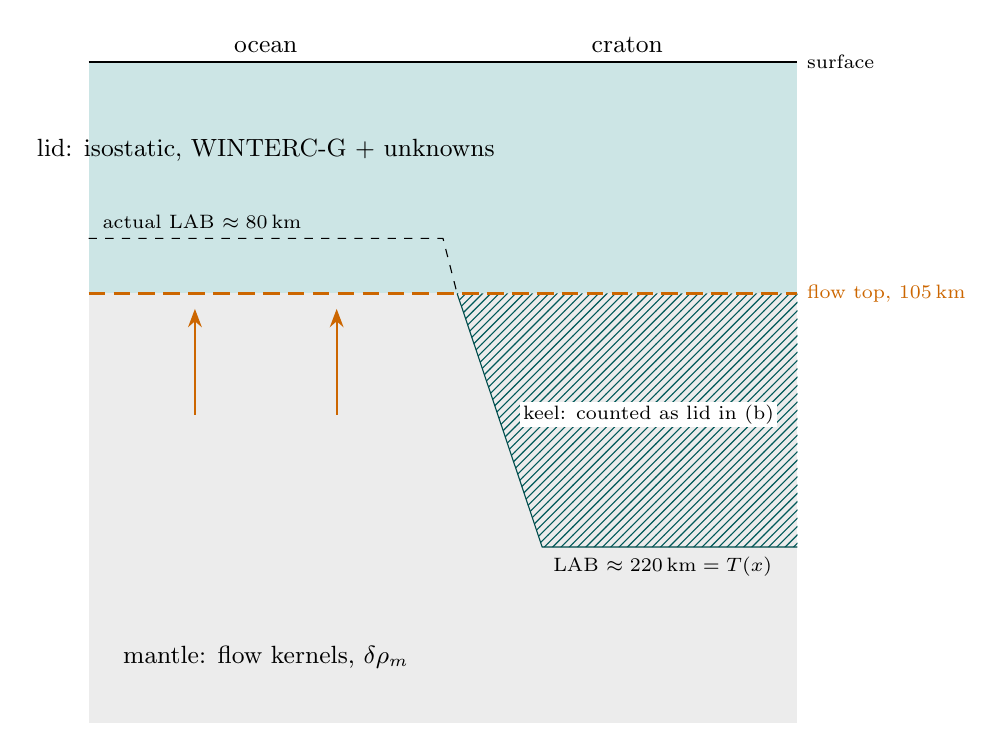
\begin{tikzpicture}[x=0.9cm,y=-0.028cm,font=\small]
\fill[gray!15] (0,105) rectangle (10,300);
\fill[teal!20] (0,0) rectangle (10,105);
\fill[pattern=north east lines, pattern color=teal!70!black] (5.2,105) -- (6.4,220) -- (10,220) -- (10,105) -- cycle;
\draw[teal!60!black] (5.2,105) -- (6.4,220) -- (10,220);
\draw[dashed] (0,80) -- (5,80) -- (5.2,105);
\draw[orange!80!black, very thick, dash pattern=on 6pt off 3pt] (0,105) -- (10,105);
\draw (0,0) -- (10,0);
\foreach \x in {1.5,3.5} \draw[-{Stealth}, orange!80!black, thick] (\x,160) -- (\x,112);
\node[above] at (2.5,0) {ocean};
\node[above] at (7.6,0) {craton};
\node at (2.5,40) {lid: isostatic, WINTERC-G + unknowns};
\node[above, font=\scriptsize] at (1.6,80) {actual LAB $\approx\qty{80}{km}$};
\node[fill=white, inner sep=1pt, font=\scriptsize] at (7.9,160) {keel: counted as lid in (b)};
\node[below, font=\scriptsize] at (8.1,220) {LAB $\approx\qty{220}{km} = T(x)$};
\node at (2.5,270) {mantle: flow kernels, $\delta\rho_m$};
\node[right, font=\scriptsize, orange!80!black] at (10,105) {flow top, \qty{105}{km}};
\node[right, font=\scriptsize] at (10,0) {surface};
\end{tikzpicture}
\caption{Option (b). The flow top stays the sphere at \qty{105}{km}; the lid base follows the LAB where it is deeper. The hatched keel moves from the mantle unknown to the lid; the mantle density is masked there.}
\end{figure}

\subsection{How WINTERC-G gets a laterally varying LAB}
WINTERC-G solves each \qty{1}{\degree} column on its own: conductive temperature to the LAB, thermodynamic densities and velocities, and elevation from isostasy.
Under isostasy a column needs only its own mass, so nothing couples it to its neighbours and the LAB can be anything at each point.
It has no flowing mantle.
Our lid works the same way, column by column, so a laterally varying LAB is just as easy there; that is (b).
Only the top of the flow domain must be a sphere, and WINTERC-G has no flow domain.
Neither model lets viscous flow go around a stiff keel.

\section{Linearisation error}

Products of perturbations are dropped.
The size of what is dropped was measured.
\begin{itemize}[nosep]
\item A finite-amplitude correction to a deflected sheet scales as $(\ell+2)\,\delta h/(2r)$: about \qty{4}{\percent} at degree 50 for a \qty{10}{km} displacement.
\item The cross term of a \qty{10}{km} Moho displacement and a \qty{30}{kg/m^3} crustal density change is \qtyrange{3}{11}{\percent} of the load (\qtyrange{70}{150}{m} of topography).
\end{itemize}
Both are documented; if the posterior moves the lithosphere far from WINTERC-G, the model should be relinearised about the posterior mean.

\begin{defence}
\Q{Why one crustal layer?}
\A It keeps the number of unknowns small and matches what the data can resolve in the topography, where only the column mass matters.
For the geoid it is a first-order limitation: moving \qty{100}{kg/m^3} between the upper and lower halves of the crust changes the geoid by about \qty{1.3}{m}, which a single uniform $\delta\rho_c$ cannot represent.
The options are a second crustal node, or carrying that effect in the modelling-error covariance.

\Q{Why three lid nodes?}
\A Three GLL nodes represent a density that varies quadratically across the lid, which is enough to capture a thermal gradient and its curvature, and the quadrature is exact for it.
The topography sees only the lid's integrated mass; the geoid sees its first moment; three nodes give the prior room for both without many unknowns.
\end{defence}

\begin{incode}{\texttt{src/density\_inversion/forward/lithosphere.py}}
\begin{itemize}[nosep]
\item \texttt{gll}, \texttt{lagrange}: the GLL nodes and weights, and the Lagrange basis on them.
\item \texttt{project\_cells}, \texttt{synthesise}: \qty{1}{\degree} cells to tapered coefficients up to \texttt{BANDLIMIT\_LMAX = 89} (\texttt{TAPER\_FROM = 70}) and back to any Gauss--Legendre grid.
\item \texttt{ReferenceLithosphere.structure}: thicknesses, contrasts and node weights at points.
\item \texttt{factor\_fields}: $f_k(x)$ in the summand order of \texttt{summands}.
\item \texttt{operator}: $(\delta\mathrm{Moho}, \delta\rho_c, \delta\rho_{\ell,n}) \mapsto q$, a row of multiplication operators.
\item \texttt{column\_mass}, \texttt{lid\_intervals}: the exact mass of each reference column, integrating WINTERC-G's piecewise-linear density piece by piece.
\item \texttt{reference\_load}: $q_{\mathrm{ref}} = -g(M - \langle M\rangle)$, the load of the reference structure itself.
\item \texttt{ocean}: the ocean function with floating ice set to 1.
\end{itemize}
\end{incode}

\chapter{The geoid of the full model}
\label{ch:geoid}

In the core model every moved mass sits either in the mantle or at the surface.
In the full model the lithosphere has structure, so the mass moved by a deflection sits at several depths, and those depths vary laterally.
This chapter explains how the geoid is computed in that case, and why the care is needed.

\section{Every mass, at its own depth}

The geoid is $N = -\Phi/g_0$ at the surface, so a mass excess raises it.
Five kinds of mass contribute.
\begin{enumerate}[nosep]
\item The mantle anomaly and the CMB it deflects, from $K_N$ (Chapter~\ref{ch:flow}).
\item The lithospheric perturbations (Chapter~\ref{ch:lithosphere}), each a sheet $\sigma(x) = f(x)\,u(x)$ at its own local depth.
\item The plate's deflection $w$: lifting a column by $w$ puts a sheet $\Delta\rho_i(x)\,w(x)$ on every density contrast $i$ of the column:
\begin{center}
\begin{tabular}{ll}
\toprule
Contrast & Sheet density per unit $w$ \\
\midrule
ice top & $\rho_{\mathrm{ice}} - \rho_w C(x)$ (where there is ice)\\
surface & $\rho_c(x) - \rho_{\mathrm{ice}}$ under ice, otherwise $\rho_c(x) - \rho_w C(x)$ \\
Moho & $\rho_{\mathrm{lid,top}}(x) - \rho_c(x)$\\
lid & the lid's own gradient, one sheet per piece between WINTERC-G knots\\
base & $\rho_{\mathrm{LAB}} - \rho_{\mathrm{lid,bottom}}(x)$, at $T$ below the column's surface\\
\bottomrule
\end{tabular}
\end{center}
These add up to $\rho_{\mathrm{LAB}}-\rho_w C(x)$, the same contrast as the plate's restoring force.
That telescoping sum is the consistency check: the total moved mass is the same in the force balance and in the geoid.
(Under floating ice, where $C=1$, the ice-top row gives $\rho_{\mathrm{ice}}-\rho_w$. Physically floating ice does not move with the bedrock, and the contrast belongs at the seafloor; the total is unchanged and the depth error is only the ice thickness.)
\item The reference lithosphere itself, a fixed term.
\item The ocean that follows the geoid (Chapter~\ref{ch:ocean}).
\end{enumerate}

\begin{decision}{Sheets at their own depth, not at a mean depth}
\textbf{Choice.} Each sheet is placed at its local depth $d_i(x)$, which varies laterally.

\textbf{Alternative.} Place each sheet at its mean depth, which keeps the operator diagonal in degree.

\textbf{Why.} The geoid of a compensated structure is a small difference between the attraction of the load and that of its compensation, so it depends on the depth difference between them.
For a Pacific-type example, the Moho sheet contributes $+17.0$ and its compensation $-17.2$\,m, a net $\qty{-0.24}{m}$.
Placing the sheets at their mean depths gives $\qty{-0.70}{m}$, three times too large.
A brute-force numerical integral gives $\qty{-0.248}{m}$.
\end{decision}

\section{Sheets at variable radius}

A sheet at radius $r(x) = R - d(x)$ has the external potential
\[
    \Phi_{\ell m}(R) = -\frac{4\pi G R}{2\ell+1}\int \sigma(x)\left(\frac{r(x)}{R}\right)^{\ell+2} Y_{\ell m}(x)\,\mathrm{d}\Omega .
\]
The factor $(r/R)^{\ell+2}$ depends on position, so it cannot be pulled out of the integral.
We expand it about a common radius $r_c$:
\[
    \left(\frac{r}{R}\right)^{\ell+2} = \left(\frac{r_c}{R}\right)^{\ell+2}\exp\!\left[(\ell+2)\ln\frac{r}{r_c}\right]
    = \left(\frac{r_c}{R}\right)^{\ell+2}\sum_{k\ge0}\frac{(\ell+2)^k}{k!}\left(\ln\frac{r}{r_c}\right)^k .
\]
Each term is a product of a known field, $(\ln r/r_c)^k\,\sigma(x)/k!$, which is expanded in harmonics once, and a degree-dependent factor $(\ell+2)^k$.
The series converges because each term is smaller by roughly $(\ell+2)|\ln(r/r_c)|/k$; $\ln(r/r_c)$ is only about \qty{1.6}{\percent} across a \qty{105}{km} column, but at high degree $(\ell+2)|\ln(r/r_c)|$ reaches about 2, so some 20 terms are needed. It is truncated at a relative tolerance of $10^{-10}$.
The method is exact for laterally varying depth, and agrees with a brute-force integral to $10^{-9}$.

\section{Two checks of the whole geoid}

\paragraph{The limit test.}
With no plate strength, water everywhere and a uniform lithosphere of density $\rho_{\mathrm{LAB}}$, all the deflection sheets collapse to a single sheet $(\rho_{\mathrm{LAB}}-\rho_w)w$.
If that sheet is moved analytically from the surface to $r_{\mathrm{top}}$, the full model must reproduce flowkernels' own geoid $K_N^{\mathrm{fk}}$ and topography $K_{h0}$.
It does, to $10^{-10}$.
This is the test that settles whether the mass removed from flowkernels' geoid and the mass added back are the same.

\paragraph{A synthetic Earth.}
For a whole synthetic lithosphere, the reference structure's own geoid has an rms of \qty{359}{m} and the geoid of its isostatic deflection an rms of \qty{346}{m}, of opposite sign; their sum has an rms of only \qty{14.8}{m}, about \qty{4}{\percent} of either part.
This shows why every per-cent-level choice in the lithosphere matters for the geoid: errors in either large term appear undiluted in the small difference.

\begin{defence}
\Q{Your reference geoid is a \qty{4}{\percent} remainder of two large terms. How can you trust it?}
\A Each term is computed exactly for the model as stated, with the sheets at their own depths, and the sum is checked against brute-force integration and against the limit test.
What is uncertain is the model, not the arithmetic: the one-$g$ approximation, the planar mass balance and the linearisation each move the remainder by up to \qtyrange{10}{15}{\percent}.
That is why the geoid's modelling error is carried as a covariance term and not ignored.

\Q{Where do you put the Moho sheet: at the unperturbed Moho or at the centroid of the perturbation?}
\A At the unperturbed Moho, which is the first-order choice.
Moving it to the centroid changes the geoid by about \qty{15}{\percent} of the total in the test case; both are second order in the perturbation, but the cancellation amplifies them.
\end{defence}

\begin{incode}{\texttt{src/density\_inversion/forward/geoid.py}}
\begin{itemize}[nosep]
\item \texttt{Geoid.sheet\_factor}: $S_\ell(r)$ per component, zero at degrees 0 and 1.
\item \texttt{sheet}, \texttt{sheets}: $\sigma\mapsto N$ for a sheet at constant radius, and for sheets at laterally varying depth (the $\ln(r/r_c)$ series).
\item \texttt{mantle\_operator}: $\delta\rho_m\mapsto N$ through $K_N$.
\item \texttt{lithosphere\_operator}: the perturbation sheets, each at its own depth (\texttt{lithosphere\_depths}).
\item \texttt{deflection\_sheets}, \texttt{deflection\_operator}: the contrasts of the table above, and $w\mapsto N$.
\item \texttt{reference\_layers}, \texttt{reference}: the reference column as exact sheets, and its own geoid.
\end{itemize}
\end{incode}

\chapter{Extension 3: the real ocean and the sea-level constant}
\label{ch:ocean}

\section{The problem}

The core model puts water everywhere; the plate of Chapter~\ref{ch:plate} puts it only in the oceans for the restoring force.
But the water that follows the geoid also has to be confined to the oceans: on land, a rise of the geoid does not add water.
Once that is so, the water's load and mass depend on $C(x)\,N(x)$, which couples degrees, and $N$ itself depends on the water.
So the geoid and the water must be solved together.

A second problem appears with real land and sea: what fixes absolute sea level?
In the core model only anomalies matter.
With a reference lithosphere and continents, the mean level of the ocean relative to the columns determines which areas are land and how high they stand, and a wrong mean produces a spurious land--ocean step.

\section{How we tackle the ocean}

The sea surface is an equipotential, so it follows the geoid: where the masses of the model raise the geoid by $N$ at sea, the water is $N$ deeper; on land nothing happens.
This is the static version of the sea-level equation of glacial isostatic adjustment, in which the ocean also follows the geoid it helps to create.

To first order the ocean that follows the geoid does two things at sea and nothing on land:
\begin{itemize}[nosep]
\item it loads the plate with its weight, $\delta q = -\rho_w g\,C N$;
\item it adds its mass to the geoid as a sheet at sea level, $\delta N = S(R)\,\rho_w C N$.
\end{itemize}
Writing $r$ for the geoid the model computes before the ocean is added (the direct geoid of all masses, plus the geoid of the deflection under their load), the total geoid satisfies
\begin{equation}
    N = r + S(R)\,\rho_w C N - G_w P\,(\rho_w g\,C N)
    \quad\Longleftrightarrow\quad
    (I + T)\,N = r,
    \qquad T = \rho_w\,(g\,G_w P - S(R))\,C,
\end{equation}
with $P$ the plate (load to deflection) and $G_w$ the geoid of the deflected column.
Both effects depend on $N$ and both change it, which is why the equation is implicit.
The water's own load and its own mass nearly cancel, as in the core model: the plate sinks under the water's weight by almost enough to remove an equal mass from the surface. So $T$ is small: its spectral radius is $0.0014$ at $L=50$.
We solve by a Neumann series, $N = \sum_k (-T)^k r$, which converges in about four terms.
The deflection is then $w = P(q - \rho_w g C N)$ and the observed topography, measured from sea level on land and at sea, $h = w - N$.

\begin{defence}
\Q{Is the self-gravitating ocean worth the trouble?}
\A The water sheet is about \qty{7}{\percent} of the mantle geoid at degree 2, though its weight sinks the plate and cancels most of that in $N$; its larger effects are on $w$ (about \qty{2}{\percent} at degree 2) and through $h=w-N$, with $N/w$ about \qty{5}{\percent} at degree 2.
Confining the water to the oceans also matters, because on land there is none.
An earlier version that took the water term from flowkernels' free-surface geoid, applied it on land as well, and never added the water's mass to the geoid had the mantle geoid \qty{11}{\percent} low at degree 2.
The fix is cheap and the limit test confirms it to $10^{-10}$.
\end{defence}

\section{How we tackle sea level}

Every column has an absolute mass per unit area, $M(x)$, from its surface to the lid base, ice included.
Heavy columns sit low and light columns stand high, but relative to what?

\begin{figure}[h]
\centering
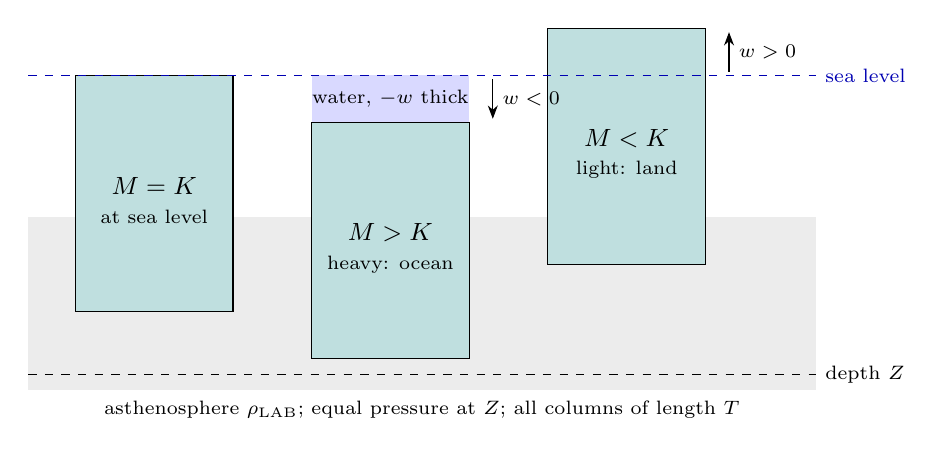
\begin{tikzpicture}[x=1cm,y=-1cm,font=\small]
\fill[gray!15] (0,3.0) rectangle (10,5.2);
\fill[blue!15] (3.6,1.2) rectangle (5.6,1.8);
\fill[teal!25] (0.6,1.2) rectangle (2.6,4.2);
\fill[teal!25] (3.6,1.8) rectangle (5.6,4.8);
\fill[teal!25] (6.6,0.6) rectangle (8.6,3.6);
\draw (0.6,1.2) rectangle (2.6,4.2); \draw (3.6,1.8) rectangle (5.6,4.8); \draw (6.6,0.6) rectangle (8.6,3.6);
\draw[blue!70!black, dashed] (0,1.2) -- (10,1.2) node[right, font=\scriptsize] {sea level};
\draw[dashed] (0,5.0) -- (10,5.0) node[right, font=\scriptsize] {depth $Z$};
\node at (1.6,2.6) {$M = K$}; \node[font=\scriptsize] at (1.6,3.0) {at sea level};
\node at (4.6,3.2) {$M > K$}; \node[font=\scriptsize] at (4.6,3.6) {heavy: ocean};
\node at (7.6,2.0) {$M < K$}; \node[font=\scriptsize] at (7.6,2.4) {light: land};
\node[font=\scriptsize] at (4.6,1.5) {water, $-w$ thick};
\draw[-{Stealth}] (5.9,1.25) -- (5.9,1.75) node[midway,right,font=\scriptsize] {$w<0$};
\draw[-{Stealth}] (8.9,1.15) -- (8.9,0.65) node[midway,right,font=\scriptsize] {$w>0$};
\node[font=\scriptsize] at (5,5.45) {asthenosphere $\rho_{\mathrm{LAB}}$; equal pressure at $Z$; all columns of length $T$};
\end{tikzpicture}
\caption{The column balance behind the sea-level constant.}
\end{figure}

Compare columns of equal length on the same asthenosphere, and require equal pressure at a depth $Z$ below them (force up = force down).
Under a column of mass $M$ whose surface is at height $w$ above sea level (positive up), the mass above $Z$ is
\[
    \underbrace{M}_{\text{column}} + \underbrace{\rho_w C\,(-w)}_{\text{water above}} + \underbrace{\rho_{\mathrm{LAB}}\,(Z - T + w)}_{\text{asthenosphere below}} .
\]
At sea $w<0$ and the water fills from the seafloor at $w$ up to sea level at 0, so its thickness is $-w$; on land $C=0$ removes the term.
Equating with the reference column ($M = K$, $w = 0$) and cancelling $\rho_{\mathrm{LAB}}(Z-T)$:
\begin{equation}
    (\rho_{\mathrm{LAB}}-\rho_w C)\,w = K - M .
\end{equation}
$K$ is a single global number, the mass a column must have to float with its surface exactly at sea level.
The per-column quantity is $K - M(x)$, the column's mass deficit or excess, and $w = (K-M)/(\rho_{\mathrm{LAB}}-\rho_w C)$ converts it into a height.

A change $\Delta K$ is not a uniform shift: it moves columns by $\Delta K/2340$ at sea and $\Delta K/3370$ on land, because water fills an oceanic deflection but not a continental one.
So a wrong $K$ creates a step between land and ocean.
In the core model, with water everywhere, the contrast is uniform and the constant $b_0$ absorbs any change of $K$, so it is not needed there.
The reference load is $q_{\mathrm{ref}} = -g(M - \langle M\rangle) + gK_0$: the mean column mass plus a constant.

\begin{decision}{Fit the sea-level constant on columns that hold their whole lithosphere}
\textbf{Choice.} $K_0$ is fitted, by least squares on the fine grid, to the observed bedrock elevation, using only columns whose WINTERC-G LAB is shallower than the column base.
A perturbation $\delta K$, with prior standard deviation \qty{1e6}{kg/m^2}, is an unknown of the inversion.

\textbf{Alternatives.} $K = \langle M\rangle$ (zero-mean load); fitting on all columns; conserving ocean mass.

\textbf{Why.}
\begin{itemize}[nosep]
\item With $K = \langle M\rangle$ there was a \qty{705}{m} spurious land--ocean step and \qty{316}{m} rms leaking into all degrees.
\item Where the LAB is deeper than the column base, the dense cold root is missing from $M$, so those columns are biased; fitting on them would push the constant to compensate.
\item After the fit, thin-lithosphere oceans match the seafloor to \qty{2}{m}, and continents stand too high in proportion to their LAB depth (\qty{+0.07}{km} for LAB $<\qty{100}{km}$, rising to \qty{+0.87}{km} beyond \qty{200}{km}): exactly the missing roots, left for the mantle unknown.
\end{itemize}
The fitted value is $K_0 = \qty{-5.2e6}{kg/m^2}$ relative to $\langle M\rangle$, equivalent to the mean column standing about \qty{2.2}{km} below sea level with the ocean contrast ($K_0/(\rho_{\mathrm{LAB}}-\rho_w)$).

\textbf{Under (b).} With the lid base following the LAB, cratons get their keels back and $K_0$ can be fitted on every column, which removes the restriction above.

\textbf{Caveat.} $\delta K$ is nearly degenerate with the degree-0 Moho displacement (correlation close to $\pm1$; with the signs used here the data constrain $\delta K - f\,\delta\mathrm{Moho}_{00}$, which gives a correlation near $+1$, whereas the audit reported $-1$: check the parameterisation), and $K_0$ is fitted to the same elevation data the inversion uses.
\end{decision}

\section{How much each part matters}
\begin{center}
\small
\begin{tabular}{p{0.28\textwidth}p{0.3\textwidth}p{0.32\textwidth}}
\toprule
& Self-gravitating ocean & Sea-level constant\\
\midrule
Question & how sea level varies with the geoid & where sea level is relative to the columns\\
Size & \qtyrange{1}{2}{\percent} of $w$ at $\ell=2$, less above; about \qty{0.1}{\percent} of $N$ & essential: \qty{705}{m} land--ocean step without it\\
Core model & simple closed form & not needed ($b_0$)\\
Could it be deferred? & yes, stating its size; but it is already built and verified & not if the final inversion uses total topography on land\\
\bottomrule
\end{tabular}
\end{center}
If the self-gravitating ocean is neglected, two things that are not really part of it must stay: water only at sea in the plate's restoring force, and $h = w - N$, because topography is measured from sea level.

\begin{incode}{\texttt{ocean.py} and \texttt{model.py}}
\begin{itemize}[nosep]
\item \texttt{SelfGravitatingOcean}: builds $T$ from $P$, $G_w$, $C$ and $S$, applies $(I+T)^{-1}$ by the Neumann series (\texttt{\_neumann}) and its adjoint the same way; \texttt{contraction} estimates the spectral radius by power iteration.
\item \texttt{ForwardModel.sea\_level\_constant}: the least-squares $K_0$ on the fine grid with area weights.
\item \texttt{ForwardModel.uniform\_load\_operator}: $\delta K \mapsto g\,\delta K$ as the degree-0 component (the orthonormal $Y_{00}$ is $1/\sqrt{4\pi}$, so a constant $c$ has component $c\sqrt{4\pi}$).
\end{itemize}
\end{incode}

\chapter{Assembly and verification}
\label{ch:assembly}

\section{The full operator}

The full model maps four unknowns to two observables:
\[
    (\delta\rho_m,\ x_L,\ h_s,\ \delta K)\ \longmapsto\ (h,\ N) .
\]
For each source $X$ of load (mantle density, lithospheric unknowns, the sea-level constant), with load operator $L_X$ and direct geoid $D_X$,
\begin{align}
    N_X &= (I+T)^{-1}\left(D_X + G_w P L_X\right) && \text{the geoid, ocean included},\\
    w_X &= P\left(L_X - \rho_w g\,C N_X\right) && \text{the deflection under its load and the water's},\\
    h_X &= w_X - N_X && \text{topography from sea level},
\end{align}
and $h = \sum_X h_X x_X + h_s + h_{\mathrm{ref}}$, $N = \sum_X N_X x_X + N_{\mathrm{ref}}$.
The reference terms $(h_{\mathrm{ref}}, N_{\mathrm{ref}})$ are the same equations applied to WINTERC-G's own load and structure: they are the fixed offset of the affine forward model.
The surface field $h_s$ is added to the topography with no load and no geoid: it is a nuisance field for short-wavelength topography that the long-wavelength model is not meant to explain, separated from the rest only by its prior, which puts its power at high degree.

\begin{incode}{\texttt{src/density\_inversion/forward/model.py}, \texttt{ForwardModel}}
\begin{itemize}[nosep]
\item \texttt{model\_space}, \texttt{data\_space}: direct sums of pygeoinf spaces, labelled.
\item \texttt{forward(x)}: $(h, N)$ including the offsets; \texttt{offset()}: the offsets alone.
\item \texttt{parts(x)}: every contribution separately (topography by source, geoid by mass), which sum to \texttt{forward}.
\item Each block is a pygeoinf \texttt{LinearOperator} with an adjoint, so the posterior can be computed matrix-free; the adjoints are consistent to $1.3\times10^{-11}$.
\end{itemize}
\end{incode}

\section{The verification}

Each check compares the code with something it does not share code with.

\begin{center}
\begin{longtable}{p{0.33\textwidth}p{0.42\textwidth}r}
\toprule
Check & Against & Agreement\\
\midrule
\endhead
Sheet factor $S_\ell$, force balances & symbolic derivation (sympy) & $3\times10^{-15}$\\
Core model & closed form & $4\times10^{-14}$\\
Topography kernels, $\ell=1$--40 & \texttt{fem\_1d}, separate finite-element code & \qty{0.09}{\percent}\\
Geoid kernels, $\ell=1$--40 & \texttt{fem\_1d} & \qty{0.1}{\percent}\\
Degree 1 & \texttt{fem\_1d} at $\ell=1$ & $10^{-4}$\\
Full model in the core limit & flowkernels' $K_N^{\mathrm{fk}}$, $K_{h0}$ & $10^{-10}$\\
Plate & manufactured solution & $10^{-9}$\\
Lithospheric load & Airy isostasy & \qty{0.06}{\percent}\\
Variable-depth sheets & brute-force integration & $10^{-9}$\\
Moved mass & mass balance (load = geoid sheets) & $10^{-9}$\\
Reference column & exact column mass & $10^{-12}$\\
Grid quadrature & refinement to $8L$ & \qty{0.2}{\percent}\\
Adjoints & $\langle Ax, y\rangle = \langle x, A^*y\rangle$ & $1.3\times10^{-11}$\\
Compensated root geoid & brute-force axisymmetric code & \qty{3}{\percent}\\
\bottomrule
\end{longtable}
\end{center}

The last row is the weakest.
The brute-force code solves the Airy balance column by column and integrates Newton's law numerically, sharing nothing with the package.
The cause of the \qty{3}{\percent} gap ($-0.240$ against $-0.248$\,m) has not been established.
Planar versus spherical mass balance is one candidate, but in the audit case it changed the result by about \qty{15}{\percent} ($-0.254$ against $-0.219$\,m), which is not obviously consistent with a \qty{3}{\percent} gap.
Until the gap is shown to shrink with resolution, describe it as an unexplained \qty{3}{\percent} disagreement, not rounding error.

\section{The approximations}

\begin{center}
\begin{longtable}{p{0.4\textwidth}p{0.45\textwidth}}
\toprule
Approximation & Size\\
\midrule
\endhead
Covariant flat plate vs thin shell & $<10^{-4}$ in $F_\ell$ for $\ell\le50$\\
Membrane stresses neglected & \qtyrange{0.2}{0.4}{\percent}\\
One $g$ in the plate and loads & \qty{0.4}{\percent} at sea\\
Radial grid of the flow kernels & $6\times10^{-4}$; up to \qty{9}{\percent} for a deep anomaly at $\ell=40$\\
First-order lithosphere & \qty{4}{\percent} at $\ell=50$ for \qty{10}{km}; cross terms \qtyrange{3}{11}{\percent}\\
Lid base fixed at \qty{105}{km} & cratons \qty{+865}{m} too high in the reference\\
One crustal layer & up to \qty{1.3}{m} of geoid\\
Ice density 910 vs 950 & documented\\
Phase-boundary deflections (410, 660) & not modelled; raised by a referee report\\
\bottomrule
\end{longtable}
\end{center}

\begin{defence}
\Q{Your radial grid converges only to first order. Is that a problem?}
\A For the topography and for degrees up to about 10 the kernels are converged to $6\times10^{-4}$.
For deep, sharp anomalies at high degree the error reaches \qty{9}{\percent}, but those combinations produce almost no surface signal.
Refinement or Richardson extrapolation is the remedy if they become important.

\Q{What about the 410 and 660 phase transitions?}
\A Their deflections are mass anomalies that the model does not represent explicitly.
To first order they behave like additional density sheets at those depths, which the mantle unknown can partly absorb; whether the prior allows it is something to test with synthetics.
\end{defence}

\chapter{The inversion framework}
\label{ch:inversion}

\section{The posterior}

With a linear forward model $d = Gm + e$, a Gaussian prior $m\sim\mathcal N(m_0, C_m)$ and Gaussian errors $e\sim\mathcal N(0, C_d)$, the posterior is Gaussian with
\begin{equation}
    \tilde C = \left(C_m^{-1} + G^{\mathsf T}C_d^{-1}G\right)^{-1},
    \qquad
    \tilde m = m_0 + \tilde C\,G^{\mathsf T}C_d^{-1}(d - Gm_0)
\end{equation}
\citep{tarantola_inverse_2005}.
Everything is exact: no sampling, no convergence to check.

\section{The evidence}

The evidence is the probability of the data under the model, with the unknowns integrated out:
\begin{equation}
    p(d) = \mathcal N\!\left(d;\ Gm_0,\ C_d + G C_m G^{\mathsf T}\right).
\end{equation}
It is computed in model space, which is small (28 scaling nodes plus the correlated field), using the Woodbury identity and the matrix determinant lemma:
\[
    \ln p(d) = -\tfrac12\Big[(d-Gm_0)^{\mathsf T}C_d^{-1}(d-Gm_0) - g^{\mathsf T}H^{-1}g
    + \ln|C_d| + \ln|C_m| + \ln|H| + n\ln 2\pi\Big],
\]
with $H = C_m^{-1} + G^{\mathsf T}C_d^{-1}G$ and $g = G^{\mathsf T}C_d^{-1}(d-Gm_0)$.
The data covariance is diagonal, so $C_d^{-1}$ and $\ln|C_d|$ are trivial; only $H$ (of model-space size) has to be factorised.

\begin{incode}{\texttt{invert\_core.py}, \texttt{Joint.solve}}
Builds $M = A^{\mathsf T}C_d^{-1}A$ and $b = A^{\mathsf T}C_d^{-1}d$ once (in \texttt{\_\_init\_\_}), where $A$ stacks the correlated-field harmonics, the scaling columns and a constant.
For each set of hyperparameters it forms the prior precision \texttt{Pinv}, adds $M$, Cholesky-factorises $H$, and returns $\ln p(d)$, and with \texttt{full=True} the posterior mean and covariance.
\end{incode}

\section{Hyperparameters}

The prior and noise models have a few parameters: the amplitude and length scale of $R(z)$, the amplitude and length scale of the correlated field, and the geoid modelling-error fraction.
We choose them by maximising the evidence (type-II maximum likelihood), within physical bounds:
\begin{center}
\begin{tabular}{lll}
\toprule
Hyperparameter & Meaning & Bounds\\
\midrule
$\sigma_c$ & pointwise sd of the correlated field & \qtyrange{10}{2000}{m}\\
$\ell_c$ & its length scale & \qtyrange{50}{5000}{km}\\
$\tau$ & geoid modelling error, fraction of observed amplitude & $10^{-3}$--3\\
$\sigma_R$ & sd of $R(z)$ about its mean & $10^{-3}$--10\\
$\ell_R$ & depth correlation length of $R$ & \qtyrange{50}{5000}{km}\\
\bottomrule
\end{tabular}
\end{center}
The bounds were added after an unbounded geoid-only fit ran off to overflow.

\begin{decision}{Type-II maximum likelihood rather than full hierarchical sampling}
\textbf{Why.} It keeps the posterior analytic and the evidence comparable across models.
\textbf{Cost.} Hyperparameter uncertainty is ignored, so posterior standard deviations are somewhat too small, and the richer model gets a few nats for free: in no-signal tests the maximised log Bayes factor reached up to about $+2$.
Bayes factors much larger than that are therefore meaningful; ones of order 2 are not.
\end{decision}

\section{The noise model for topography}

\paragraph{Thinning.}
Holdt's 10,874 oceanic points are averaged in \qty{1}{\degree} cells, giving 7,434 cells.
The error of a cell is the rms of its points' errors, not reduced by $\sqrt n$, because residuals of nearby points are correlated (correlation 0.63 within \qty{25}{km}, near zero beyond \qty{100}{km}): averaging correlated errors does not reduce them by $\sqrt n$.

\paragraph{The correlated field.}
Residual depths contain signal the mantle term cannot produce (unmodelled crust, the lithosphere's own variation, errors in the corrections), and it is spatially correlated.
Leaving it out would force the mantle term to fit it, or would make the errors look independent when they are not.
We add a field $c(x)$ of degrees 1--40, with a Sobolev-type spectrum $\propto(1 + (\ell_c/b)^2\ell(\ell+1))^{-2}$ normalised so that its pointwise standard deviation is $\sigma_c$, and integrate it out.

\paragraph{The constant.}
Residual depths are relative to an age--depth curve, whose zero is arbitrary; a constant $b_0$ (prior sd \qty{1000}{m}) is fitted.

\section{The noise model for the geoid}

The geoid product gives coefficients at degrees 2--25 with variances from the satellite model, the crustal correction and the LAB correction, plus the hydrostatic term, for which we use the uncertainty of \citet{chambat_flattening_2010} (\qty{1}{m} on $C_{20}$, \qty{0.2}{m} on $C_{40}$).
$C_{21}$ and $S_{21}$ are removed, because they are dominated by the rotational pole, not the mantle.

\begin{decision}{Diagonal geoid covariance plus a modelling error}
\textbf{Choice.} Use the diagonal of the stated covariance, floored at 0.2 times the median within each degree, and add $\tau^2$ times the observed power at each degree.

\textbf{Why.} The product's low-rank covariances are each the mean of only 2--4 difference vectors, so they assert exact correlations and leave some combinations of coefficients with only the satellite variance, about $10^{-13}\,\mathrm{m}^2$: the inversion then fits those combinations exactly.
The modelling-error term represents geoid structure that a single 1D scaling cannot produce; without it the geoid-only $R(z)$ oscillated wildly to fit noise.
\end{decision}

\section{The prior on $R(z)$}

$R(z)$ is given on 28 nodes (\qty{105}{km}, then \qtyrange{200}{2800}{km} every \qty{100}{km}) with hat functions in between.
Its prior has a squared-exponential correlation in depth plus a common offset with standard deviation $\sigma_\mu = 1$ that is marginalised:
\[
    C_R = \sigma_R^2\exp\!\left[-\tfrac12\left(\frac{z_i-z_j}{\ell_R}\right)^2\right] + \sigma_\mu^2\,\mathbf 1\mathbf 1^{\mathsf T},
    \qquad m_0 = 0.
\]
The offset term means the prior does not force $R$ towards zero on average; it lets the data choose the mean level, while $\sigma_R$ controls variation about it.

\section{The mantle unknown in the final inversion}
In the final inversion the mantle density $\delta\rho_m(r,x)$ is itself the unknown, a full 3D field with of order $10^4$ coefficients; no scaling of tomography is imposed.
\begin{center}
\small
\begin{tabular}{lll}
\toprule
& First inversion (core) & Final inversion\\
\midrule
Mantle unknown & $R(z)$, 28 numbers & $\delta\rho_m(r,x)$, a 3D field\\
Lateral pattern from & tomography, fixed & the data and the prior\\
Lithosphere & corrected in the data & unknowns about WINTERC-G\\
Data & oceanic residual depths, geoid & total topography everywhere, geoid\\
\bottomrule
\end{tabular}
\end{center}
The data give at most two numbers per $(\ell,m)$, so the null space is large and the depth distribution of density comes almost entirely from the prior.
The prior is an open decision:
\begin{enumerate}[nosep]
\item \textbf{zero mean, Sobolev covariance}: the data alone choose the pattern; cleanest, poorest depth resolution;
\item \textbf{scaled tomography as the prior mean}, $m_0 = \rho_0\,\hat R(z)\,\mathrm{dlnV_s}$ with $\hat R$ from the first inversion: the final inversion then asks where the mantle departs from the scaling once the lithosphere is modelled, which links the two inversions; it inherits tomography's errors where the data are silent;
\item \textbf{tomography in the covariance only}, for example a larger variance where $|\mathrm{dlnV_s}|$ is large.
\end{enumerate}

\section{Testing whether the fit means anything}

\paragraph{The Bayes factor.}
The log Bayes factor of the scaling model against a null model ($R=0$, same noise model) is the difference of their log evidences.
A value of 5 means the data are $e^5\approx150$ times more probable under the scaling; on the scale of \citet{kass_bayes_1995}, $\ln B$ of 3--5 is strong and above 5 very strong. With the offset prior $\sigma_\mu=1$ fixed, the Bayes factor also contains an Occam factor that depends logarithmically on $\sigma_\mu$, so state that value whenever you quote a Bayes factor.

\paragraph{The rotation null.}
A large Bayes factor could arise because any smooth field with the right spectrum helps, not because the tomography's geography is right.
To test that, we rotate all predicted node fields by the same random rotation of the sphere, which keeps their spectra and depth structure but destroys their alignment with the data, and refit.
If the geography matters, the rotated fits should do much worse than the unrotated one; they do (log Bayes factors $-5.6$ to $-3.3$ against $+35.2$).

\begin{defence}
\Q{Isn't the correlated field just absorbing the signal?}
\A It overlaps strongly with the mantle term: each mantle column lies \qtyrange{98.7}{99.2}{\percent} in the span of the field's harmonics.
So ``variance explained by the mantle'' means the share assigned to the mantle under the fitted priors.
The Bayes factor and the rotation null are what show that the mantle term is doing something the field cannot.

\Q{Why point evaluation rather than spherical harmonic coefficients of the data?}
\A Because the data are points with individual errors and large gaps.
Expanding them into coefficients first would need interpolation into the gaps and would turn independent errors into correlated ones.
Evaluating the prediction at the points keeps the data as they are.
\end{defence}

\chapter{The first inversion: a single 1D scaling}
\label{ch:single}

\section{The question}

The simplest link between seismic tomography and density is a single radial scaling,
\[
    \delta\rho_m(r,x) = \rho_0(r)\,R(r)\,\mathrm{dlnV_s}(r,x),
    \qquad R = \frac{\mathrm d\ln\rho}{\mathrm d\ln V_s},
\]
the same everywhere at a given depth.
The question is whether such a scaling, applied to a modern tomography model, explains oceanic residual depths and the geoid, and with which $R(z)$.
Its failure, if it fails, is the motivation for the perturbation formulation about WINTERC-G.

\section{Why the old run was replaced}

An earlier version of this inversion, using a forward operator built with the HC code, gave an oscillating $R(z)$ and $\chi^2/\nu\approx30$.
Reviewing it showed:
\begin{itemize}[nosep]
\item its predicted topography for a plausible $R=0.25$ was 4.5--23 times too large and anticorrelated with the data ($r=-0.17$ to $-0.26$), too large in amplitude and of the wrong sign, so the oscillation was the fit fighting the operator;
\item it included a flexural restoring term with $\rho_m-\rho_l = \qty{400}{kg/m^3}$, which is wrong for water-loaded seafloor;
\item it used the posterior of the earlier chapter as data, which shrinks to zero where there are no data; predicting zero topography already scored 36.5 per degree of freedom;
\item the HC output's Condon--Shortley phase is mislabelled in its docstring (it is $+1$), found by checking that cratons come out fast.
\end{itemize}
The rerun replaces it with the core model, the data points themselves, and the noise model of Chapter~\ref{ch:inversion}.

\section{Set-up}

\begin{itemize}[nosep]
\item \textbf{Tomography.} SL2013sv \citep{schaeffer2013global} above \qty{660}{km}, S40RTS \citep{ritsema_s40rts_2011} below \qty{1008}{km}, with a $\cos^2$ taper between, on layers every \qty{100}{km}, rebuilt from the HC repository files (reproducing the saved blend to $6\times10^{-9}$).
\item \textbf{Forward model.} The core model with the $\times30$ viscosity jump, degrees 1--31 (the tomography's maximum).
\item \textbf{Topography.} Holdt's oceanic residual depths (7,434 cells), with the correlated field and $b_0$.
\item \textbf{Geoid.} Degrees 2--25 of the geoid product, diagonal errors plus $\tau^2$ modelling error.
\item \textbf{Prior.} $R(z)$ on 28 nodes, as in Chapter~\ref{ch:inversion}.
\end{itemize}

\section{Results}

\begin{center}
\begin{tabular}{lrp{0.5\textwidth}}
\toprule
Data & ln BF & $R(z)$ and fit\\
\midrule
Topography & $+35.2$ & $+0.08$ at \qty{105}{km}, $\approx0$ at \qtyrange{300}{400}{km}, $+0.18$ at \qtyrange{1700}{2000}{km}; variance reduction 0.22, correlation 0.46\\
Geoid & $+96.4$ & oscillating; $-0.97\pm0.12$ at \qty{105}{km}; variance reduction 0.37\\
Joint & $+10.8$ & smooth ramp $+0.01$ to $+0.15$; topography VR 0.12, geoid VR $-0.02$\\
Rotation null (topography) & $-5.6$ to $-3.3$ & 6 rotations\\
\bottomrule
\end{tabular}
\end{center}

Without degree 1 the topography gives $+39.0$ and the joint $+13.8$, with similar $R(z)$.

\section{Reading the results}

\begin{enumerate}[nosep]
\item \textbf{A 1D scaling of the tomography is strongly supported by the residual depths.}
A log Bayes factor of 35 against the null, and $-3$ to $-6$ for rotated predictions, means the geography of the tomography matters.
\item \textbf{But it explains only about a quarter of their variance, with small $R$.}
Values of \numrange{0.05}{0.2} are smaller than those usually assumed for a purely thermal origin \citep[e.g.][]{karato1993importance,cammarano2003inferring}; check the ranges in those papers before quoting a comparison.
\item \textbf{The geoid wants something quite different near the top.}
A strongly negative $R$ at \qty{105}{km} would mean fast regions are \emph{light}.
Taken literally, $R\approx-1$ means $\delta\rho/\rho\approx-\mathrm{dlnV_s}$, about \qty{-150}{kg/m^3} for a root \qty{5}{\percent} fast: far more than chemical depletion can supply (tens of \si{kg/m^3}).
More likely the top node is absorbing something else: errors in the crustal and LAB corrections already applied to the geoid, or geoid structure a 1D scaling cannot fit.
It is a symptom, not a measurement.
\item \textbf{No single $R(z)$ serves both.}
The joint fit is a compromise that explains none of the geoid.
Our working hypothesis is that the conflict sits at the top of the mantle, where the lithosphere is; this is not yet demonstrated.
A test would be a joint fit in which the geoid has its own $R$ at the \qty{105}{km} node, or one with that node removed: if the joint Bayes factor recovers, the conflict is at the top.
\end{enumerate}
This is the argument for the perturbation formulation: the lithosphere's density is not a fixed scaling of its velocity, so it must be modelled explicitly, and the mantle below it inverted as a perturbation.

\begin{defence}
\Q{A Bayes factor of 35 but only \qty{22}{\percent} variance explained: which is it?}
\A Both.
The Bayes factor measures whether the scaling helps relative to no mantle term, given the noise model; the variance reduction measures how much of the data it accounts for.
A model can be decisively better than nothing and still leave most of the signal unexplained.

\Q{Is the geoid's negative $R$ just an artefact of the oscillation?}
\A The geoid-only $R$ does oscillate, and its fine structure should not be interpreted.
Possibly. The posterior standard deviation at that node, 0.12, is small, but a small standard deviation on one node of an oscillating profile does not make it robust: it is conditional on the hyperparameters and on the noise model.
Nor is $R\approx-1$ a natural mantle value: the isopycnic hypothesis \citep{jordan1978composition}, in which composition offsets temperature in cratonic roots, predicts $R\approx0$, not $-1$, and the reference lithosphere elsewhere in this guide suggests the deep roots are net dense.
The safest reading is that the geoid alone cannot be fitted by a 1D scaling near the top, and the top node takes up the misfit.

\Q{How robust is this to the viscosity and the tomography?}
\A In the earlier full-model run, viscosity variants changed the log Bayes factor between 30 and 35 and tomography models between 17 and 21.
Repeating these with the core model is on the to-do list.
\end{defence}

\begin{incode}{\texttt{scripts/single\_scaling/}}
\begin{itemize}[nosep]
\item \texttt{build\_core.py}: the core operator (Chapter~\ref{ch:core}).
\item \texttt{invert\_core.py \{topo,geoid,joint\}}: thinning, geoid data, the \texttt{Joint} evidence, the fit, and the summary JSON.
\item \texttt{rotate\_null.py}: the rotation null.
\item Results: \texttt{outputs/single\_scaling/result\_core\_*.json} and \texttt{posterior\_core\_*.npz}; the no-degree-1 runs are kept with suffix \texttt{\_nodeg1}.
\end{itemize}
\end{incode}

\chapter{The decision ledger}
\label{ch:ledger}

Every modelling decision in one place: what was chosen, the evidence for it, and the caveat to state.

\begin{center}
\small
\begin{longtable}{p{0.22\textwidth}p{0.38\textwidth}p{0.3\textwidth}}
\toprule
Decision & Evidence & Caveat\\
\midrule
\endhead
Linear--Gaussian & exact posterior and evidence; flow linear in $\delta\rho$ & viscosity fixed per run; lithosphere linearised (Ch.~\ref{ch:lithosphere})\\
Build the forward model up in stages; two inversions (core, full) & each stage checked against the previous by forward comparison; core vs full: $r\ge0.996$, \qtyrange{1}{4}{\percent} at ocean points & changes between the two inversions not attributable by inversion alone\\
Compressible, self-gravitating flow & standard since \citet{corrieu_mantle_1995}; negligible cost & comparison with incompressible studies needs care\\
Sparse BVP, not propagators & no exponential ill-conditioning; matches \texttt{fem\_1d} to \qty{0.1}{\percent} & radial grid first-order\\
Free slip, flow top at \qty{105}{km} & mean WINTERC-G LAB \qty{102}{km} & \qty{28}{\percent} of area has a deeper LAB\\
$\times30$ jump at \qty{670}{km} & log BF 30--35 across variants (full model) & density depends on viscosity: adjoint kernels\\
Degree 1 included & \texttt{fem\_1d} agreement $10^{-4}$; real data & lowers BF 39.0 $\to$ 35.2\\
Moved mass at the surface & mass at \qty{105}{km} gave geoid wrong by 0.2--3$\times$ & ---\\
Water follows the geoid; $h = w - N$ & \qty{2}{\percent} of $w$ at $\ell=2$; $N/w\approx\qty{5}{\percent}$; limit test $10^{-10}$ & net effect on $N$ only \qty{0.1}{\percent}\\
Elastic plate on land and sea & land deflection otherwise 1.44$\times$ too large & $T_e$ matters above $\ell\approx20$ (\qty{22}{\percent} at $\ell=40$ for \qty{80}{km})\\
Deflection kept on the fine grid & truncation loses \qtyrange{10}{23}{\percent} of the geoid & ---\\
WINTERC-G reference & consistent crust + lid densities globally & circular: fitted to elevation and gravity\\
One crust layer, three lid nodes & topography sees only column mass & up to \qty{1.3}{m} of geoid from crustal layering\\
$\delta$LAB dropped & double counting where LAB $>\qty{105}{km}$ & ---\\
Lid base at \qty{105}{km} (current) & matches flow top; inherited from the core model & cratons \qty{+865}{m} high in the reference; keels treated as fluid\\
Lid base $T(x)=\max(105, \mathrm{LAB})$ with a mantle mask (planned, (b)) & keel counted once, in the lid; no solver change & flow not deflected around keels; oceanic asthenosphere above \qty{105}{km} still lid\\
Flow top a sphere at \qty{105}{km} & per-degree solver needs spherical boundaries & lateral viscosity would need a 3D solver\\
Sheets at their own depth & mean-depth error $3\times$ (\qty{-0.70}{} vs \qty{-0.24}{m}) & ---\\
$K_0$ fitted on thin-lithosphere columns & removes \qty{705}{m} land--ocean step & fitted to the same data; degenerate with Moho$_{00}$\\
Point evaluation of topography & keeps errors independent & thinning to \qty{1}{\degree} cells\\
Correlated field in the noise & residual correlation 0.63 within \qty{25}{km} & overlaps the mantle term (\qty{99}{\percent})\\
Diagonal geoid errors + $\tau^2$ & low-rank covariances near-singular ($10^{-13}$) & ---\\
Type-II ML hyperparameters & keeps evidence analytic & sds too small; ln BF $\lesssim2$ not meaningful\\
Rotation null & rotated fits $-5.6$ to $-3.3$ vs $+35.2$ & 6 rotations so far; run $\sim$50\\
\bottomrule
\end{longtable}
\end{center}

\section{The questions most likely to come up}

\Q{In one sentence, what does your forward model do?}
\A It computes the instantaneous flow driven by a mantle density anomaly in a compressible, self-gravitating Earth with radial viscosity, and from it the deflection of an elastic lithosphere floating in a self-gravitating ocean, and the geoid of every mass that moves.

\Q{Why should I believe topography breaks the depth degeneracy?}
\A It doesn't break it on its own: each kernel is a depth average.
What helps is that the two kernels have different depth shapes (topography one-signed and largest when shallow; the geoid changing sign with depth and degree), that their shapes change with degree, and that $R(z)$ is assumed common to all degrees.
In particular, a shallow dense anomaly and a deeper light one can give the same geoid but give topography of opposite sign.

\Q{What is the weakest part of the model?}
\A The lithosphere: the reference model was fitted to the same kind of data, the lid base is fixed at \qty{105}{km} although cratonic roots go deeper, and the geoid of the lithosphere is a small remainder of large terms.
That is why the first inversion uses only oceanic data and the core model, and why the full model carries a modelling-error covariance.

\Q{What would change your conclusions?}
\A A different viscosity profile changes the recovered density (quantified by the adjoint kernels); a different reference lithosphere changes the continental results; a deeper lid base moves cratonic signal from mantle to lithosphere.
How sensitive the oceanic single-scaling result is to these has only been tested with the earlier full model (viscosity: log Bayes factor 30--35; tomography: 17--21), and still needs repeating with the core model.

\Q{Why not use a 3D viscosity?}
\A Lateral viscosity variations couple every degree to every other, so the per-degree solver no longer works and each column of the operator needs a 3D Stokes solve.
For a fixed viscosity field the problem would still be linear in density; the costs are computation, the loss of the exact per-degree kernels on which the viscosity kernels rely, and a new uncertain input (the keel's viscosity).
Lateral variations are a known limitation, partly represented by the lithosphere being a separate elastic layer and, in (b), by keels being carried isostatically in the lid.

\Q{How do you know the code is right?}
\A Every component agrees with something independent: closed forms, symbolic algebra, a separate finite-element code, brute-force integrals and conservation laws (Chapter~\ref{ch:assembly}).
An independent audit found errors, and each was fixed with a test that would catch it again.

\section{Limitations and future work}
What can be deferred, and at what cost:
\begin{center}
\small
\begin{longtable}{p{0.3\textwidth}p{0.3\textwidth}p{0.3\textwidth}}
\toprule
Item & Cost of deferring & Status\\
\midrule
\endhead
Shallower flow top (\qtyrange{50}{60}{km}) & oceanic asthenosphere stays in the lid & future work\\
Second crustal node & up to \qty{1.3}{m} of geoid from layering & future work, or modelling-error covariance\\
Lateral viscosity & flow not deflected around keels & future work (3D solver)\\
Relinearisation about the posterior & a few per cent where the posterior moves far & future work\\
Self-gravitating ocean & \qtyrange{1}{2}{\percent} of $w$ at $\ell=2$ & deferrable with its size stated (already built; to discuss with David)\\
Lid base at the LAB, (b) & cratons \qty{+865}{m} high in the reference & deferrable only with a lid-depth sensitivity test and no interpretation beneath cratons\\
Plate on land and sea & land wrong by a factor 1.44 & not deferrable if continents are used\\
Sea-level constant & \qty{705}{m} land--ocean step & not deferrable if continents are used\\
\bottomrule
\end{longtable}
\end{center}
The key decision is whether the final inversion includes continents; most of the complexity follows from it.

\appendix
\chapter{Conventions}
\label{app:conventions}

\begin{center}
\small
\begin{longtable}{p{0.25\textwidth}p{0.68\textwidth}}
\toprule
Quantity & Convention\\
\midrule
\endhead
Stress & positive in tension; $\sigma_{rr}$ from flowkernels' traces, non-dimensional, times $\eta_{\mathrm{ref}}/r_{\mathrm{top}}$\\
Potential & physics sign, $\nabla^2\Phi = 4\pi G\rho$, so $\Phi<0$ near a mass; Corrieu's $U = -\Phi$\\
Geoid & $N = -\Phi/g_0$ at $r=R$; a mass excess raises $N$\\
Load $q$ & \si{Pa}, positive up; a mass excess gives $q<0$\\
Deflection $w$ & m, positive up; the radial motion of the column\\
Topography $h$ & $h = w - N$, measured from sea level (orthometric), on land and at sea\\
Interface perturbation & positive up; $\Delta\rho_i = \rho_{\mathrm{below}} - \rho_{\mathrm{above}}$; relative to the plate\\
Depths in WINTERC-G & positive down from sea level; bedrock elevation positive up\\
Reference column & from the column's own surface to $T=\qty{105}{km}$ below it\\
Harmonics (package) & real, orthonormal on the unit sphere ($\int Y^2\,\mathrm d\Omega = 1$), Condon--Shortley phase $+1$ (pyshtools \texttt{norm=4, csphase=1})\\
Component order & degree by degree; orders $0, 1..\ell, -1..-\ell$\\
Sphere spaces & unit radius; components are orthonormal coefficients; plate rigidity passed as $D/R^4$\\
Geoid product & orthonormal, Condon--Shortley phase $-1$, radius $a = \qty{6378136.3}{m}$, degrees 2--25; convert by $(-1)^m (R/a)^{\ell-1}$\\
HC tomography & dlnVs in per cent; \texttt{hc\_io} output is csphase $+1$ although its docstring says $-1$\\
Degree 0 & excluded from the mantle and geoid; constants fitted separately ($b_0$, $\delta K$)\\
Degree 1 & centre-of-mass frame: $N_1=0$; load and topography at $\ell=1$ kept, $h_1=w_1$\\
Gravity & $g_{\mathrm{LAB}} = \qty{9.91}{m/s^2}$ for loads and the plate; $g_0 = GM/R^2 = \qty{9.82}{m/s^2}$ for the geoid\\
Densities & $\rho_w = \qty{1030}{kg/m^3}$; $\rho_{\mathrm{ice}} = \qty{910}{kg/m^3}$; $\rho_{\mathrm{LAB}}$ from PREM at the flow top\\
Ocean function & $C=1$ at sea and under floating ice, 0 on land\\
Viscosity & 1 above \qty{670}{km}, 30 below (jump on the node at \qty{666}{km})\\
RMS of a field & $\sqrt{\sum c_{\ell m}^2/(4\pi)}$ over the chosen degrees\\
\bottomrule
\end{longtable}
\end{center}

\paragraph{Still to reconcile.}
The chapter's definition of topography (Eq.~\texttt{topo-definition}) must be checked against $h = w - N$ with $w$ from $q = (\rho_{\mathrm{LAB}}-\rho_w)gw + \dots$, which in the project notes is written $h = -\tau_b/(\Delta\rho\,g_0)$ with $\tau_b$ in tension: with $\tau_b = \sigma_{rr}$ at the flow top and $q=-\sigma_{rr}$, the two agree in sign only. They differ by $g$ versus $g_0$ and by the $-N$ term in $h=w-N$ (a few per cent at low degree).

\chapter{Where everything lives}
\label{app:files}

\begin{center}
\small
\begin{longtable}{p{0.45\textwidth}p{0.48\textwidth}}
\toprule
Path & What it is\\
\midrule
\endhead
\multicolumn{2}{l}{\textbf{\texttt{density-inversion/src/density\_inversion/forward/}}}\\
\texttt{mantle.py} & flow kernels from flowkernels (Ch.~\ref{ch:flow})\\
\texttt{plate.py} & elastic plate, land and sea (Ch.~\ref{ch:plate})\\
\texttt{lithosphere.py} & lithospheric unknowns and WINTERC-G reference (Ch.~\ref{ch:lithosphere})\\
\texttt{surface.py} & the surface field $h_s$\\
\texttt{geoid.py} & every mass's geoid (Ch.~\ref{ch:geoid})\\
\texttt{ocean.py} & the self-gravitating ocean (Ch.~\ref{ch:ocean})\\
\texttt{model.py} & assembly, sea-level constant (Ch.~\ref{ch:assembly})\\
\texttt{examples.py} & conversions between coefficient conventions\\
\multicolumn{2}{l}{\textbf{\texttt{density-inversion/scripts/single\_scaling/}}}\\
\texttt{build\_core.py} & the core operator (Ch.~\ref{ch:core})\\
\texttt{invert\_core.py} & evidence, fit, results (Ch.~\ref{ch:inversion}, \ref{ch:single})\\
\texttt{rotate\_null.py} & the rotation null\\
\texttt{build\_operator.py}, \texttt{invert.py} & full-model operator, older inversion, shared helpers (nodes, hats, harmonics)\\
\multicolumn{2}{l}{\textbf{Elsewhere}}\\
\texttt{density-inversion/tests/} & the verification tests; \texttt{test\_mantle.py} includes the \texttt{fem\_1d} check for $\ell=1$--40\\
\texttt{density-inversion/notes/audit/} & findings, convention ledger, justification notes, referee reports\\
\texttt{density-inversion/outputs/single\_scaling/} & operators, posteriors, result JSONs\\
\texttt{products/geoid\_for\_inversion.npz} & the geoid data and its variances\\
\texttt{data/hoggard/global.xyz} & residual depths: first 4,119 rows Stephenson (continents), the rest Holdt (oceans)\\
\texttt{data/hc/} & HC tomography and viscosity files, blend script\\
\texttt{ch3-overleaf} (branch \texttt{main}) & the chapter on Overleaf\\
\texttt{ch3-drafts/drafts/} (branch \texttt{claude}) & Claude's reference drafts and notes\\
\bottomrule
\end{longtable}
\end{center}


\bibliographystyle{plainnat}
\bibliography{refs}
\end{document}
